% !TEX root = MasterThesis.tex

\chapter{Modern Operating System Concepts}\label{ch:modern-os-concepts}
This thesis' introduction already picked up the discussion about which operating system architecture is the superior one by referring to the \textit{Tanenbaum-Torvalds debate}\cite{linux-is-obsolete} in 1992.
Besides the discussion is quite interesting from today's view on different operating systems, the forecasts on their future and the actual development, are both, \textsc{Tanenbaum} and \textsc{Torvalds} underpinning their arguments with the origins of their implementations \textit{MINIX} and \textit{Linux} in different problems. 
And roughly spoken are exactly such different problems which needs to be solved with an operating system one reason for their diversity. 
Over the years, they had to fit in solving very different kinds of problems on very different kinds of hardware, which resulted in many ways of working and architectures. 
As with the debate, it is rather difficult to impossible to find one architectural concept or implementation which is clearly superior to the other ones in every use-case. 
Nevertheless, it is a reasonable question why a majority of the operating system kernels which were developed from scratch in the last few years are based on a microkernel concept.
In 2009, the official statement of the Linux kernel developer \textsc{Richard Gooch} was still that monolithic kernels are superior for performance reasons\cite{why-linux-monolith}.
So the question remains what changed during the last ten years to promote this change, and especially for this work, how this affects device driver development.
For this reason, this chapter is dedicated to the basic components and functionalities of operating system kernels and how they are implemented in the real world examples \textit{Linux} and \textit{Zircon}.

\section{Operating System Architectures}\label{sec:kernel-arch-concepts}

% TODO OS design goals see Betriebssysteme Glatz 
As already pointed out are architectural decisions for operating systems commonly influenced by the issues they are intended to solve.
By giving priority to some design objectives that are pertinent to the underlying issue, different concepts and architectures are the outcome.
According to \textsc{Glatz}\cite{glatz2015betriebssysteme} are some of them:
\begin{itemize}
    \item Providing a reliable, crash-proof environment.
    \item Providing a portable operating system.
    \item Providing a scalable operating system, e.g.\ in terms of processing cores.
    \item Providing an extensible operating system, e.g.\ in terms of adding additional functionality to the kernel.
    \item Providing real-time capabilities.
    \item Providing an efficient design in terms of resources and performance.
    \item Providing a secure environment for user applications.
    \item Providing a maintainable operating system, e.g.\ by the division of policy and mechanism. 
\end{itemize}\ \\
%
In addition, operating systems should also pay attention to the common software design issue \textit{mechanism vs.\ policy}.
That means an operating system design should provide a clear distinction between the \textit{mechanism}, that means the capable abilities that can be performed (how is something done) and the \textit{policy}, which controls how the available capabilities are used (what is done)\cite{lfd430},~\cite{silberschatz2009operating}.
An example for driver development could be controlling the number of processes that can use a device at once.
In this case, the driver should provide the mechanism, \textit{how} such a limitation could be done, but not \textit{what}, the actual number of allowed processes. 
The idea behind is that requirements may change over some time and such a distinction makes it easy to adjust the \textit{policy} via some parameters without touching the underlying \textit{mechanism}\cite{silberschatz2009operating}.

How these design principles fit into the known operating system architectures will be considered in the following sections.
But before, the terms' \textit{kernel mode} and \textit{user mode} will be explained as they are fundamental for this work.

\subsubsection*{Dual-Mode Execution}
Modern general purpose \acp{cpu} provide a ring based, hardware enabled security model which had its origin in the Intel x86 processor architecture\cite{tanenbaum-modern-operating-systems}.
It is usually made of four different security levels, the rings 0 to 3 which are illustrated in Figure~\ref{pic:x86rings}.
In this theoretical model, ring 3 is the least secure level, used for common user applications (even if started with extended privileges (\textit{root} for the UNIX-like world)), while ring 2 is used for libraries shared between user applications and ring 1 is for system calls\cite{glatz2015betriebssysteme}.
Actual operating system implementations may not use all of them.
Linux for example utilize ring 3 for user-space applications, shared libraries and ring 0 for system calls and the kernel.
System calls provide the transition to ring 0, the one with the topmost security level, which is used for the operating system kernel.
Actual operating system implementations may not use all of them.
Linux for example utilize ring 3 for user-space applications, shared libraries and ring 0 for system calls and the kernel.
As a crucial part of an operating system, system calls will be discussed in more detail later in this work.

Directly related to this model is the \textit{dual-mode} execution mode of modern \acp{cpu}.
It is a hardware enabled security concept to provide a distinction between the user applications in ring 3 and the actual operating system kernel in ring 0.
Just the kernel in ring 0, running in the \textit{kernel mode} (or \textit{privileged mode, supervisor mode or system mode}), has direct and privileged access to memory, hardware, timers or interrupts, e.g.\ for performing \ac{io} operations or memory mappings\cite{lfd430}.
User applications in ring 3, running in the \textit{user mode}, are not allowed to them so directly, they have limited privileges and a limited instruction set.
As named above, they need to use a mechanism called \textit{system calls} to transfer the execution to the \textit{kernel mode} where the privileged actions are performed.
Lastly, the execution is transferred back to the calling user process and with this, the mode changes back to \textit{user mode}.
Figure~\ref{pic:mode-switches} pictures the operating flow of a system call including the mode switches between \textit{user} and \textit{kernel mode}.

%
%
\begin{figure} [ht]
	\centering
	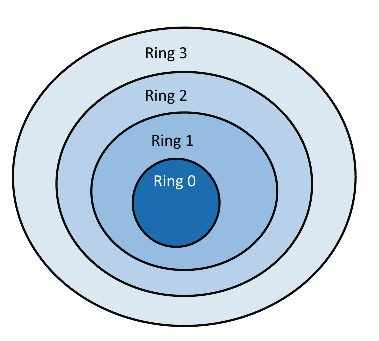
\includegraphics[scale=0.6]{x86Rings}
	\caption{The Rings of the x86's security concept\cite{glatz2015betriebssysteme}}\label{pic:x86rings}
    %TODO own picture!
\end{figure}
%
\begin{figure} [ht]
	\centering
	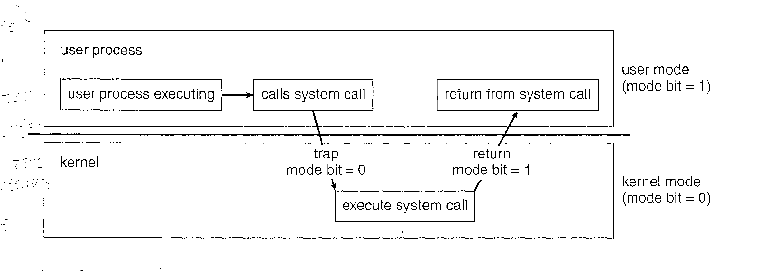
\includegraphics[scale=0.6]{mode-switch}
    \caption{A system calls sequence including the mode switches\cite{glatz2015betriebssysteme}}\label{pic:mode-switches}
    %TODO own picture!
\end{figure}

The \ac{cpu}'s operating mode is usually controlled by a specific bit in the \ac{psw}\cite{tanenbaum-modern-operating-systems}.
\ac{psw} is term on x86 \ac{cpu} architectures. 
It is corresponding to the \ac{cpsr} on ARM architectures\footnote{http://infocenter.arm.com, visited on 08.03.2019 \url{http://infocenter.arm.com/help/index.jsp?topic=/com.arm.doc.dui0473f/CHDFAEID.html}}.
But since in literature is always spoken of the \ac{psw} regardless of the concrete \ac{cpu}'s architecture, this should also be done in this work.
It influences the state of each \ac{cpu} core itself in a multi-processor system, but not the operating system kernel.
As a result, different \ac{cpu} cores may be in a different execution mode\cite{lfd430}.
With this separation, any privileged instruction is forbidden in \textit{user mode} and will not be executed.

Based on the dual mode execution on the \ac{cpu}, different architectural concepts for operating systems evolved.
They differ e.g.\ in the share of the operating system respectively the operating system's kernel actually running within the \ac{cpu}'s \textit{kernel mode}. 
Thus, they have an influence on the whole system, including device driver development but also on performance and security issues.

With this basic knowledge about the \ac{cpu}'s operating modes, the next section researches a selection of different operating system architectures.
Special attention should be paid to the most common ones, the \textit{monolithic} and the \textit{microkernel} architectures and their implementation in Linux and Zircon.
On the contrary, this work will not take a particular look on special purpose operating system architectures such as ones for loosely coupled multi-processor systems known from processing clusters.
Today, even the majority of general purpose computing systems are driven by more than one \ac{cpu} cores and most of common modern operating systems are designed to provide support for the de facto standard for tightly coupled systems, \ac{smp}.


\subsection{Monolithic Architectures}\label{sec:monolithic-archs}
Some sources, such as \textsc{Glatz}\cite{glatz2015betriebssysteme} or \textsc{Silberschatz}\cite{silberschatz2009operating}, suggest monolithic operating systems do not have a well-defined structure at all. 
As they are indeed most commonly grown structures, started in a completely different scope (MS-DOS, the original UNIX), it is not an incorrect claim.
But it does not necessarily have to be the case.
Above all, monolithic operating system (kernel) architectures have in common that they form one single binary program which is running entirely in kernel mode.
User programs, running in user mode, interact with the kernel only through a well-defined set of \textit{system calls}\cite{lfd430}. 
Within the kernel itself, all parts are free to use and access each other but also the hardware, without any limitation, e.g.\ regarding the access of kernel functionalities of another component or hardware access. 
That means a function or procedure initial developed for scheduling processes could be used in a completely different context if its functionality is useful to solve another issue.
In fact, there is no information hiding between kernel functions or procedures.
Any function in this kernel context has full access to the hardware, such as \ac{io} devices, timers, interrupts and even to the memory. 
There is no memory protection or validation between different components of a monolithic kernel. 
Of course, this leads to some serious disadvantages in this architecture, for example could a crash in one single function or procedure crash the entire kernel or the resulting system may become difficult to understand and maintain\cite{tanenbaum-modern-operating-systems},~\cite{silberschatz2009operating}.
The missing memory protecting within the kernel could also be a source for crashes or attacks.
But in contrast, this design also enables a very efficient kernel design without any unneeded communication overhead or hardware inefficiencies\cite{lfd430}.

An extension of the monolithic architecture are the so-called \textbf{modular operating systems}.
They provide additional, defined interfaces for (in common) dynamically loadable and unloadable extensions, e.g.\ for device drivers or filesystems. 
Sometimes, such extensions or modules are just allowed to use a limited function set of the operating system, but they are still running as a part of the kernel in kernel mode\cite{lfd430},~\cite{tanenbaum-modern-operating-systems}. 
Just like ordinary kernel functions or procedures, (malicious) programming errors in extensions may lead to a kernel crash or manipulate or damage other components.
Contrary, the modular concept provides some advantages over regular monolitic kernels.
It allows slimming down the actual kernel by providing the chance to reload only the actually needed functionality dynamically and e.g.\ security patches within such an extension is possible without restarting the entire system\cite{brause2017betriebssysteme}.
As the extensions become a part of the operating system running in kernel mode, no additional communication effort between the actual kernel and the modules is required.
Thus, concept of modules is quite popular for basically monolithic operating systems like \textit{Linux} or \textit{Solaris}\cite{brause2017betriebssysteme},~\cite{silberschatz2009operating}.


\subsection{Microkernel Architectures}\label{sec:microkernel-archs}
The microkernel architecture focuses on very opposite design goals compared to the monolithic one. 
Some of them are to cope the complexity, rather poor maintainability and susceptibility to errors by a massively modular approach. 
To archive this, the core idea behind microkernels is to provide only a very small kernel running in kernel mode which only provides the core functionalities while all the other important functions of an operating system are running in user mode.
Thereby, the microkernel architecture is excellently suited to implement a proper division of mechanism and policy.
The kernel provides just the most basic mechanisms needed for an operating system, while the userspace modules implement the policy.
This decoupling makes it easier to change the policy in userspace for altering requirements without touching the actual kernel\cite{tanenbaum-modern-operating-systems}.

What is part of this core functionality differs between miscellaneous sources, but all considered ones are in agreement that a simple mechanism for process scheduling is as well a core functionality as providing an \ac{ipc} mechanism\cite{lfd430},~\cite{silberschatz2009operating},~\cite{glatz2015betriebssysteme}.  
In contrast, the sources disagree whether memory management and virtualization, device drivers or synchronization facilities are a part of the actual kernel.
The \textit{Mach} microkernel, which formed the first generation of microkernels in 1985, named process and thread administration, an extensible and secure \ac{ipc} mechanism, virtual memory management and scheduling as its core tasks, while everything else needed has to run in usermode\cite{rashidMach}.
Functional enhancements of the system do not require changes to the kernel itself, too.
This concerns, depending on the exact realization, device drivers, memory management, system call handlers and even more system components\cite{lfd430},~\cite{silberschatz2009operating}.
In academic microkernel approaches, all components in user mode run within an own userspace process as small, well-defined modules, while the communication is done through copious message passing via the actual kernel\cite{tanenbaum-modern-operating-systems},~\cite{lfd430}.
Since the restrictions by the \ac{cpu}'s dual mode still apply for microkernel based operating systems is it not allowed to device drivers running in user mode to have direct physical access to \ac{io} ports as a consequence.
A device driver has to invoke the actual kernel to perform the needed action substitional.
But thus, the kernel is able to check the action and whether the driver is authorized to executed them.
Resulting, the microkernel design is more reliable and secure as such a division enables the kernel to intercept erroneous actions such as accidental memory writes to important regions\cite{tanenbaum-modern-operating-systems}.
Equally, a crash in a userspace system component like a driver is not able to crash the entire kernel in such an approach. 
And as an additional advantage facilitate the microkernel architecture porting the operating system kernel to another target architecture as the most hardware dependencies are part of the small kernel\cite{silberschatz2009operating},~\cite{lfd430}.

With all the named advantages microkernels offer, the question remains why microkernels are only spread in real-time, avionics or military but not for desktop operating systems.
One reason is that all these advantages are bought at the high price of microkernel message costs.
For the named application areas, especially the reliability that comes with the microkernel architecture is more desirable than the performance costs of the lot more context switches in comparison to monolithic architectures\cite{tanenbaum-modern-operating-systems}.
Since a lot of the operating system's functionality has been moved to the userspace, microkernel architectures need to perform noticeable more context switches to invoke the actual kernel for privileged actions. 
The performance losses are not only caused by the large amount of context switches themselves, but also by the fact that modern \acp{cpu}, particularly the caches are not designed for them. 
Every context switch causes cache misses which trigger that the required data has to be loaded from the slower main memory and cached. 
The data of the previous context (e.g.\ the user mode context) will be displaced from the cache and the \ac{cpu} is largely blocked in the meantime.
By rapidly switching back to the previous context, as is usual for e.g.\ a short kernel invocation to perform an \ac{io} operation on microkernel architectures, the cache is no longer suitable for the new context and has to be replaced\cite{lfd430}.

First of all, the \textit{L4} kernel, a second generation microkernel was able to get close to the performance of a monolithic kernel as \textit{Linux} it is\cite{Hrtig1997}.   
This has been achieved by improving the \acf{ipc} mechanism, a fundamental component of microkernel architectures on which other communication mechanisms are based.
% by improving ipc performance, only synchronous ipc
Nevertheless, are pure microkernels mainly used for systems with high reliability requirements but unusual for desktop application. 
Some industry examples are \textit{Integrity}, \textit{QNX} and \textit{seL4}, a mathematically verified version of the \textit{L4} kernel\cite{tanenbaum-modern-operating-systems}. 

%TODO ? reincarnation server : check if all modules are up running and work correctly -> if not it replaces them without user interaction \cite{tanenbaum}
%TODO picture \cite{microkernels}


\subsection{Layered Architectures}
Layered operating system architectures are usually organized in hierarchical layers, but sometimes the chosen model is described as a series of concentric rings.
Each layer or ring provides a group of functionality while it is only allowed to use the functions of the one directly below. 
The cooperating between the layers or rings is regulated by clearly defined interfaces\cite{brause2017betriebssysteme}.
This is usually accompanied by the fact that the lower layers or inner rings are more privileged as the outer ones.
However, there is no uniform and universally accepted approach for division in layers and their count according to this pattern\cite{glatz2015betriebssysteme},~\cite{tanenbaum-modern-operating-systems}.
In fact, a meaningful division is not that easy.
Functionalities may have to be divided artificially and the harmonious arrangement can have its pitfalls caused by the access requirements this architecture is based on.
Is the layered access model considered properly to get a clean architecture, it that can unfold its advantages.
These are for example the interchangeability of the layers if they and their interfaces were properly designed or the resulting concept for debugging.
As the layers are constructed on top of each other, it is possible to debug  and verify each one for its own, starting at the lowest layer up to the top most one\cite{silberschatz2009operating}.
But also the costs for system calls are comparatively high, because they have to be passed though all layers while each one adds overhead to such a call\cite{silberschatz2009operating}.  

In general, layered operating system architectures are related to monolithic ones, but it is conceivable to adopt the idea for microkernel approaches, e.g.\ is the MINIX userspace divided into layers. 
Examples for this architecture are \textit{OS/2} or newer \textit{Unix} variants, while \textit{Multics} is one for a concentric ring based model\cite{glatz2015betriebssysteme},~\cite{tanenbaum-modern-operating-systems}.


% \subsection{Distributed Architectures}


\subsection{Hybrid Architectures}
Hybrid operating system architectures based on monolithic, microkernels and may be the layered ones are common approach to combine the advantages of these concepts.
They try to pair the performance of the monolithic design with the modularity and reliability of microkernels\cite{microkernels},~\cite{silberschatz2009operating}.
How both worlds interact is very different depending on the exact implementation.
\textsc{Silberschatz} explains one of them in his book \textit{Operating System Concepts}\cite{silberschatz2009operating} using Apple's \textit{OS X} (today named \textit{macOS}) as an example.
Depending on the exact implementation and the share of the architectures, most disadvantages of monolithic architectures still apply for the hybrid systems.
Further examples for hybrid architectures are \textit{Windows NT} and \textit{BeOS}\cite{microkernels}.  


\subsection{The Linux Kernel's Monolithic Architecture}

Linux is the perfect example for an extremely grown operating system.
Starting as a pure hobby project to learn about a specific \ac{cpu} and connect to the Unix computers at \textsc{Linus Torvalds}, its initial author's, university, it becomes strongly related to its archetype, \textit{Unix}\cite{DiamondTorvalds2002}. 
They share fundamental design goals, just like being capable of multiple processors and user at the same time, but Linux is not based on the origin Unix source code\cite{tanenbaum-modern-operating-systems}.
The overall architecture of the Linux kernel is, as already named, monolithic and also inspired by Unix\cite{lfd430},~\cite{DiamondTorvalds2002}.
It is entirely running in kernel mode and all built-in layers have full access to the internal kernel \ac{api} using common function calls like in C.
A sophisticated concept of kernel modules which can be dynamically loaded to a running kernel makes a limited number of microkernel advantages available for Linux.
Modules in Linux are only allowed to use a restricted (exported) set of functions to use, but once loaded to the running kernel, they become a part of the monolith running in kernel mode\cite{lfd430}.
Linux is largely compatible to the \ac{posix} standard which was initially created for Unix.
Initially, it was because \textsc{Torvalds} could not get a version of the standard, while today it is rather a conscious decision\cite{DiamondTorvalds2002},~\cite{tanenbaum-modern-operating-systems}. 
Also, the decision for the monolithic architecture is today consciously supported by the kernel community and justified with its performance and efficiency over microkernels due to the \textit{privilege barrier} between user and kernel mode which has to be passed quite often in microkernel architecture\cite{why-linux-monolith},~\cite{lfd430}.
The Linux kernel itself is divided in five essential tasks which are also reflected in its source code.
They are: 
\begin{itemize}
    \item Process Management,
    \item Memory Management,
    \item Filesystems,
    \item Device Management and
    \item Networking\cite{lfd430}.
\end{itemize}
By structuring this tasks and further components into \textit{subsystems} like \textit{drivers/}, \textit{fs/} (filesystems), \textit{net/} or \textit{kernel/}, the Linux kernel remains comprehensible and in some ways modular. 
A closer look to the most of them in general but also their implementation in Linux is done in the following sections.

The Linux kernel is mainly written in C but some very hardware dependent part are in Assembly. 
Additionally, especially the Assembly parts were strongly dependent on the \ac{gcc}.
Today, there are some efforts to reduce the share of Assembly for maintenance and readability since modern compilers do not generate less efficient code as hand-written Assembly is\cite{programming-religion}.
This also reduces the dependency to \ac{gcc} and enables the use of alternative compilers, especially Clang\cite{linux-clang},~\cite{fosdem-linux-llvm}.
Nevertheless, the Linux kernel's principal language is C and it only provides support for C drivers. 


\subsection{The Zircon Kernel's Microkernel Architecture}
% design goals, architecture, interface posix, parts, language/compiler
In contrast to the Linux kernel, Zircon is not a grown structure.
Started in 2015, it was largely developed from scratch by Google for a so far undisclosed field of application\cite{chat-zircon-arch}.
Nevertheless, Zircon emerged from a branch of \textit{Little Kernel} (LK) by \textsc{Travis Geiselbrecht} which is also a part of the Zircon Team at Google\cite{zircon-vs-lk}. 
Despite its origin, Zircon is very different to Little Kernel.
It targets powerful devices such as modern computers and phones and provides for this reason only 64-bit support, first class user-mode support and a capability-based security model. 
In contrast, Little Kernel is designed for embedded applications and amongst others used as bootloader for \textit{Android} and as \textit{Android Trusted Execution Environment (Trusty TEE)}\cite{lk-intro}.
It has 32-bit support, but none of the more sophisticated features Zircon has\cite{zircon-vs-lk}.

The mirokernel architecture is justified by having security, safety, reliability and modularity as major design goals for Zircon.
According to \textsc{Travis Geiselbrecht} was the architecture a conscious tradeoff between the named goals and performance\cite{chat-zircon-arch}.
They try avoid costly context switches as much as possible, speed up the remaining ones and take advantage from \ac{smp}, but it is not the focus of Zircon.
Alike, Zircon does not focus on performing \ac{io} operations or process management which are the key tasks \ac{posix} was designed for\cite{chat-zircon-arch}.
As a result, Zircon does not claim to be or to become \ac{posix} compatible, they just support a very basic subset of the standard\cite{zircon-libc-posix}.
% For \ac{ipc} Zircon provides a mechansim based on an \ac{idl} which is widly used within the Zircon kernel but also in Fuchsia as the whole operating system.
The Zircon kernel itself is splitted up into the actual microkernel running in kernel mode (\textit{kernel/}) and services, drivers and core libraries running in user mode (\textit{system/})\cite{zircon-intro}.
The kernel part provides the basic operating system mechanisms: 
\begin{itemize}
    \item Process Management,
    \item (virtual) Memory Management,
    \item \acl{ipc} and
    \item Synchronization Mechanisms\cite{zircon-intro}.
\end{itemize}
The part running in user mode contains core services for, amongst others, booting, device management and networking, device drivers respectively hardware related code and user libraries.

Zircon is for the most parts written in C++ and less in C.
It provides native support for device drivers in both languages but due to the fact Zircon provides an \ac{idl} which defines a contract for in-process drivers, other languages are conceivable as well.
In fact, support for Rust drivers is currently being worked on\cite{chat-zircon-arch}.
Unlike Linux, Zircon provided support for both, the \ac{gcc} and the Clang compiler, from the beginning caused by the sophisticated tools around Clang and LLVM\@.


\section{System Calls}\label{sec:system-calls}
System calls were already marginally mentioned in this work as the mechanism to switch the program execution between user and kernel mode, because  applications running in user mode have only restricted rights.
Thus, this special calls are needed for the interaction with basic hardware devices like the \ac{cpu}, the memory, peripherals or filesystems and for invoke the actual operating system's kernel for management operations like process management\cite{lfd430}. 
System calls are to a high degree hardware dependent and differ between various operating system implementations.
% Even operating systems which comply the \acf{posix} standard may differ in the typ and number of available system calls.
% The wide-spread \ac{posix} standard is only an \ac{api} definition but not one for system calls.
% An operating system may implement the \ac{posix} standard functions within a library which often involve system calls, but it has not to do so\cite{lfd430},~\cite{glatz2015betriebssysteme}.
% Equally, a system is not constrained to a single \ac{api} and may implement different ones using its existing set of system calls\cite{glatz2015betriebssysteme}.
% \ac{posix} is implemented is a very common standard which is for example implemented in UNIX, macOS, MACH and partly in Linux\cite{tanenbaum-modern-operating-systems},~\cite{glatz2015betriebssysteme}.
% Another example for an \ac{api} is Win32 used by Windows to abstract their system calls.
% As a result system calls are rarely used directly by user applications without an abstraction layer such as libraries. An example is the \textit{libc}\cite{lfd430},~\cite{tanenbaum-modern-operating-systems}.
%

A system call has its origin in an application running in user mode.
If the application has to invoke the operating system kernel, e.g.\ to perform an action on memory in substition, it has to use one for switching the operating mode\cite{glatz2015betriebssysteme},~\cite{tanenbaum-modern-operating-systems}.
As switching the \ac{cpu}'s execution mode also means a new context, a system call to the kernel differs from a common procedure call.
In user mode, the so-called entry code stores the system call's parameters in a defined way.
One is to store the parameters and the call's number in defined registers (see~\ref{pic:syscalls}), another one is to store them on stack, according the C/C++ calling in reverse order\cite{silberschatz2009operating},~\cite{glatz2015betriebssysteme}.
The exact one depends on the actual \ac{cpu} architecture.
The following instruction triggers a special software interrupt containing the order to switch the context.
It is also named \textit{trap instruction}\cite{glatz2015betriebssysteme},~\cite{tanenbaum-modern-operating-systems}.
To be exact, it is the interrupt vector number of the trap instruction which is responsible for the switch.
They are \texttt{0\x80} on Linux as pictured in~\ref{pic:syscalls} and \texttt{0\x2e} on Windows systems\cite{glatz2015betriebssysteme}.
But right before switching it is needed to save the \acf{psw}, which contains the actual processors state includes the mode bit, to the stack.
The same number is used in kernel mode as an index within the interrupt vector table (or interrupt descriptor table, IDT) which contains the start address of the system service dispatcher routine (compare to~\ref{pic:syscalls}).
This tables content, the system service dispatcher routine, is loaded as next instruction to the new \ac{psw}\cite{brause2017betriebssysteme}.
Jumping to this routine, the system call's parameters and its number are restored to examine the actual call and invoke the matching service routine from the system service dispatching table which finally fulfills the requested action as simplified pictured in~\ref{pic:syscalls}\cite{glatz2015betriebssysteme}.
Conclusively, the control flow jumped back to the system service dispatcher which hands the control back to user space including switching back to user mode in the common way to return\cite{glatz2015betriebssysteme}.
The previous \ac{psw} is restored from stack containing the bit for \ac{cpu}'s user mode execution.
The user application has to clean up the stack like for each procedure call at the very end\cite{tanenbaum-modern-operating-systems}.

Figure~\ref{pic:syscalls} shows a simplified version of the system call implementation on x86 for Linux kernel before 2.5\cite{decade-linux-syscalls}.
More modern versions use the special instructions \texttt{SYSENTER} and \texttt{SYSEXIT} (Intel) or \texttt{SYSCALL} and \texttt{SYSRET} (AMD) instead of the slower trap interrupts\cite{decade-linux-syscalls}.

\begin{figure} [ht]
	\centering
	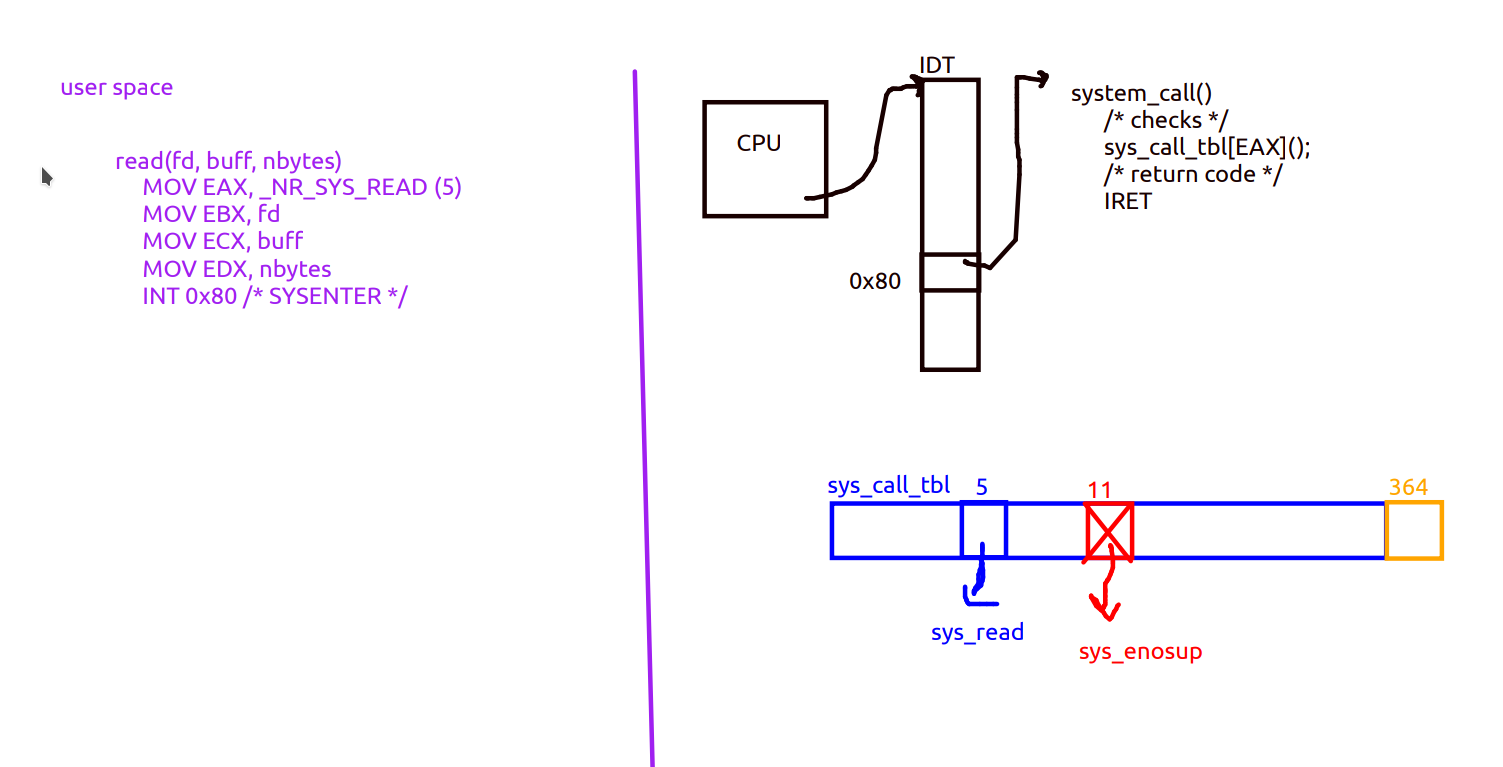
\includegraphics[scale=0.4]{syscall-lfd}
    \caption{System Call Implementation\label{pic:syscalls}\cite{lfd430}}
    %TODO own picture!
    %TODO add numbers and a kind of flow sequence with numbers. Add numbers to text.
\end{figure}


\subsubsection{POSIX}
The basic idea behind the \acf{posix} standard is to define a stable interface between the user-space and the operating system kernel to achieve portability for applications on systems meeting this standard.
But even if an operating system comply them, it may differ in the type and number of available system calls.
\ac{posix} is only an \ac{api} definition but not one for system calls.
An operating system may implement the \ac{posix} standard functions within a library which often involve system calls, but it has not to do so\cite{lfd430},~\cite{glatz2015betriebssysteme}.
System calls are rarely used directly by user applications without an abstraction layer such as libraries. An example is the \textit{libc} on Unix-like systems\cite{lfd430},~\cite{tanenbaum-modern-operating-systems}.
Equally, a system is not constrained to a single \ac{api} and may implement different ones using its existing set of system calls\cite{glatz2015betriebssysteme}.

\ac{posix} is a very common standard which is for example implemented in UNIX, macOS, MACH and partly in Linux\cite{tanenbaum-modern-operating-systems},~\cite{glatz2015betriebssysteme}. 
Another example for an \ac{api} is Win32 used by Windows to abstract their system calls, but as a result, applications targeting the Windows Win32 \ac{api} are not portable to systems implementing the \ac{posix} standard.
% As a result system calls are rarely used directly by user applications without an abstraction layer such as libraries. An example is the \textit{libc}\cite{lfd430},~\cite{tanenbaum-modern-operating-systems}.


\subsection{System Calls in Linux}
In fact, the way system calls are working in Linux was already described as part of the general section. 
The exact mechanism, the calling convention but also the number of system calls is highly depending on the \ac{cpu}'s architecture.
While a 32-bit Linux kernel in version 4.8 for the x86 architecture offered 379 calls, the 64-bit version for x86\_64 offered only 328\cite{lfd430}.
The \textit{man-pages} project documents gives an overview (\texttt{man 2 syscall}) about architectural differences and the calling conventions.
How far Linux is actually compatible to the \ac{posix} standard is not only related to the kernel and the number of system calls itself, but for the most part to its abstraction layer, the used \ac{posix}/C standard library.
One of the most spread ones, the \textit{glibc} (GNU C Library) aims to follow POSIX.1\-2008 amongst other standards\footnote{\url{https://www.gnu.org/software/libc/}} while the \textit{musl} library does not implement it in complete\footnote{\url{https://repo.or.cz/w/musl-tools.git/blob_plain/HEAD:/tab_posix.html}}.



\subsection{System Calls in Zircon}
% FIDL, core libs,.. 
% http://research.cs.queensu.ca/~cordy/Papers/BKBHDC_ESE_Linux.pdf
% for vdso
In Zircon, system calls are bounded to the concept of \textit{handles}, a construct which allows applications running in user mode to reference an object in kernel mode\cite{zircon-handle}.
Interactions between user applications and kernel objects are still done using system calls but the most of them are using a handle which describes the kernel object to work on\cite{zircon-concepts}. 
Handles are checked by the kernel each time a system call is triggered.
For additional security, the kernel checks whether
\begin{itemize}
    \item a handle has the correct type for the system call, 
    \item a kernel handles parameters refers to one existing within the calling process's handle table and
    \item a handle has the necessary rights for the triggered action\cite{zircon-concepts}.
\end{itemize}
% 
In contrast to Linux, Zircon provides just one library for system calls and the standard C implementation, the \textit{libzircon.so}.
It is a \acf{vdso} directly provided by the kernel and not stored as a physical \ac{elf} file on disk.
For the reason that \acp{vdso} are accessible from both, kernel and user mode, without switching the context, they are a perfect concept to implement system calls in a very performant way\cite{vdso-linuxjournal}.
Thus, the Zircon \ac{vdso} is the only way to perform system calls\cite{zircon-vdso}, which is a very elegant solution to cope with performance issues in a microkernel architecture.

The system calls are defined by using an abstract definition syntax and the matching tool \textit{abigen} which generates header files and code for the libzircon and the kernel's system call implementation\cite{zircon-concepts}.
Also in contrast to Linux does Zircon respectively Fuchsia not aim for \ac{posix} compatibility.
It implements only a very limited subset of \ac{posix} consisting of basic \ac{io} operations and pthreads.
Zircon does not support Unix-like signals, symbolic links and much more\cite{zircon-libc-posix}.
The libzircon.so does not support directly \ac{io} operations. 
They are performed by the \textit{fdio.so} library which overwrites weak symbols of the libzircon\cite{zircon-libc-posix}.
All available system calls in Zircon from the version this thesis is working on are documented in \url{https://github.com/Allegra42/zircon/tree/i2c-grove-lcd/docs/syscalls}. 

\section{Processes and Threads}\label{sec:processes-threads}

Modern operating systems are characterized by their ability to perform various tasks at the same time.
So far, this fact has simply been accepted within this work, but it was not questioned what is special about it and how this multitasking is achieved by an operating system.
In general, parallelization of tasks can take place on different levels, e.g.\ as hardware or software parallelism.
While the physical resources for the first case are actually available to execute the tasks really simultaneously, it only seems to be so for software parallelism\cite{glatz2015betriebssysteme}.
Hardware parallelism is realized by independent, may specialized execution units such as multiple processing cores or controllers which are able to perform particular parallel to the main \ac{cpu}.
This could be USB, network or graphics controller, for example\cite{glatz2015betriebssysteme}.
In order to create the impression of parallelism on a single \ac{cpu} and to use their available computing power as good as possible, an abstraction to provide pseudo concurrency for the execution of several tasks is required.
According to \textsc{Tanenbaum}, this concept called \textit{process model}, is the most central one of operating systems\cite{tanenbaum-modern-operating-systems}.
The term \textit{process} is often defined as a program in execution\cite{achilles2006betriebssysteme}.
The process model is complemented by the thread model which provides a simplified version for parallelism within a process or an application\cite{glatz2015betriebssysteme}.
The following sections take a closer look at these concepts and answer the remaining questions, in particular about the process and thread model, synchronization mechanisms, inter process communication and their implementation in Linux and Zircon.


\subsection{Processes}
% model, what is a process
% \cite{glatz2015betriebssysteme}:
% each process has virtually the whole cpu and corresponding resources for itself (cpu, register, address space)
% process model realizes/coordinates the parallel execution of more than one process -> time multiplexing
% reality: num processes > num cpu cores -> pseudo parallel execution
%
% \cite{tanenbaum-modern-operating-systems}: process model
% runnable software is organized as a number of sequential processes, process is an instance of an executing program including its current values (pc, registers, variables) -> each one has its own virtual cpu -> real cpu switches different processes -> called multiprogramming
%
% programm needs to be in a defined format (object file format)
% \cite{silberschatz} program is a passive entity -> executable file, process is an active entity (pc, ...)
%
% -> vordergrund/hintergrundprozesse (ui, deamon processes)
% foreground(background) background -> not associated with users but with specific function -> deamon (accept incomming mail, ..) \cite{tanenbaum-modern-operating-systems}

% process implementation

% process is different in different systems -> needs something like a processor control block (pcb) (containing all relevant data, an id (pid), process state, process context,...)
% -> for a parallel execution we need to switch between them -> context switches
% process needs to be paused and resumed -> relevant information needs to be stored and restored -> cpu register contents (pc, sp, psw), process relevant memory contents (stack), register contents are copied to pcb and restored from there, memory content stays -> each process gets a private part of the memory
%
% \cite{achilles2006betriebssysteme}  process contains memory segments -> programm code, data segement(s), stack, heap + exclusive resouces and if cpu is active -> cpu register -> saved in pcb if process is interrupted (contains id, priority, process rights, maximum resources (max cpu time, max files open, ..), actual resources (actual cpu time, ...)
%
% \cite{tanenbaum-modern-operating-systems}
% process table -> one entry per process (process control block) -> contains information about the process's state (pc, stack pointer, memory allocation, status of open files, accounting and scheduling information, priority, pid, parent process, ...)
%
% \cite{silberschatz}
% pcb: process state (running, waiting,...), program counter, cpu registers, cpu scheduling information, memory management information, accounting information (maximum and actual cpu time used, time limits, account numbers, ..), io status information (io devices, open files, ... allocated by this process)
%
% process states
% \cite{tanenbaum-modern-operating-systems} process states
% running actually using cpu
% ready runnable, temporary stopped to run other process
% blocked unable to run until sth external happens, e.g. a resource is freed
%
% \cite{silberschatz}
% new -> process is being created
% running ->
% waiting -> (blocked)
% ready
% terminated
%
% % lifecycle
% \cite{mandl2014Grungkurs}
% pic mandl
% pic silberschatz
% 1 os activates process
% 2 os interrupts other process/ preemption
% 3 process is blocked (waits for input, resources)
% 4 reason for blocking is not longer available -> resources are available
% 5 process is terminated (in(voluntary))
% -> pic tanenbaum

% multiprogramming model

% programm needs to be in a defined format (object file format)
%
% \cite{tanenbaum-modern-operating-systems}
% improves cpu utilization
% - hardware stacks pc, ...
% - hardware loads new pc from interrupt vector
% - registers are saved
% - new stack is setuped
% - interrupt service runs (reads and buffers input)
% - scheduler decides which process is to run next
% - new process is started
% process start
% \cite{glatz2015betriebssysteme}, \cite{tanenbaum-modern-operating-systems}
% process start:
% -system start (initialisation)
% -system service call for process creation (through a running process)
% -application start (via user)
% - init batch job
%
% -> vordergrund/hintergrundprozesse (ui, deamon processes)
% foreground(background) background -> not associated with users but with specific function -> deamon (accept incomming mail, ..) \cite{tanenbaum-modern-operating-systems}
% types of new processes
% process chaining -> unix exec
% process forking -> unix fork
% process creation -> (threads pthread create, win thread create), win process create
% % data for new processes
% data for new process -> inherit of all data (need to share same programm code), data buffer which is init via old process (via ipc), new process with initial values e.g. via sys call params
%
% inherit -> fork, win createprocess (\cite{achilles2006betriebssysteme}: both processes running at the same time, or parent waits for child to be ended, both share all resources/ a part of them /none, address space: child is a duplicate of parent/ child runs a new programming)
% ipc -> unix popen
% initial params -> posix pthread create, win create thread
% % process termination
% \cite{glatz2015betriebssysteme}, \cite{tanenbaum-modern-operating-systems}
% termination:
% - normal exit (voluntary)
% - ahead of time , error exit (self detected error, voluntary)
% - ahead of time (fatal error, detected by system) (not voluntary)
% - terminated/killed by other process (not voluntary involuntary)


The term \textit{process} describes an instance of a program in execution, including all its required resources to enable a model for the pseudoparallel execution of multiple programs based thereon\cite{silberschatz2009operating},~\cite{tanenbaum-modern-operating-systems}.
Each program in execution is modeled as a separate process which is assigned to a virtual private \ac{cpu} including \ac{cpu} registers, above all the program counter (PC) and a virtual private address space\cite{tanenbaum-modern-operating-systems}.~\cite{glatz2015betriebssysteme}.
Especially by using virtual private memory, processes are not only modeled individually, but are also isolated from each other in reality in order to prevent errors or deliberate attacks between programs\cite{brause2017betriebssysteme}.
But since in reality more processes, respectively programs, have to be executed than \acp{cpu} exists, a mechanism is needed to switch between processes and allow the execution of all them.
This mechanism behind, the \textit{multiprogramming model}, and the policies called \textit{process scheduling} will be considered hereafter.

However, for a change between the execution of programs to succeed, a process must contain information about its state at the moment it is interrupted to run another one.
Which information need to be stored and the way it is done slightly depends on an effective system's design and its implementation.
In general, these informations are stored in a structure called \textit{process control block} in literature\cite{tanenbaum-modern-operating-systems}.
Depending on the implementation, it contains for example
\begin{itemize}
    \item a process id, 
    \item the process's state,
    \item the \ac{cpu}'s register contents, especially the program counter (PC), the stack pointer (SP) and the processor status word (PSW),
    \item the process's address space including the program code, its stack and heap and data segments, 
    \item information about resources allocated by the process like open files, or \ac{io} devices,
    \item \ac{cpu} scheduling and accounting information like a priority, the maximum and actual computing time for this process,
    \item the parent process and
    \item the process's rights\cite{tanenbaum-modern-operating-systems},~\cite{glatz2015betriebssysteme},~\cite{achilles2006betriebssysteme},~\cite{silberschatz2009operating}.
\end{itemize}

\subsubsection*{Process Lifecycle}
The state in the list above refers to a process's lifecycle.
It is quite easy and in most cases described as a state chart like pictured in figure~\ref{pic:process-lifecycle}.
Once a process was created, it is managed by the operating system and changes its state to \textit{ready}.
The process is ready to run, but has to wait until the system allocates a \ac{cpu} to it.
Is that the case, the process changes its state to \textit{running} and performs its calculations.
If a process is interrupted (preempted) by the operating system without having fulfilled its task completely, there can be two reasons for this which result in different subsequent states.
Was the process interrupted just to run another one, the process's state changes back to \textit{ready}. 
It only lacks on \ac{cpu} time to run the process again.
If the reason was instead that resources like the process is waiting for an external event or required \ac{io} devices are used by another process, so it changes its state to \textit{waiting} or \textit{blocked}. 
Only when the blocking resource needed by the process is available again, the operating system changes the status of the process to \textit{ready} again.
The process is prepared to get reassigned to a \ac{cpu}.
A running process finishing its task during its computing time has reached the end of its life, its state changes to \textit{terminate}.
The operating system destroys the process and frees related resources\cite{silberschatz2009operating},~\cite{mandl2014Grundkurs}.

\begin{figure} [ht]
	\centering
	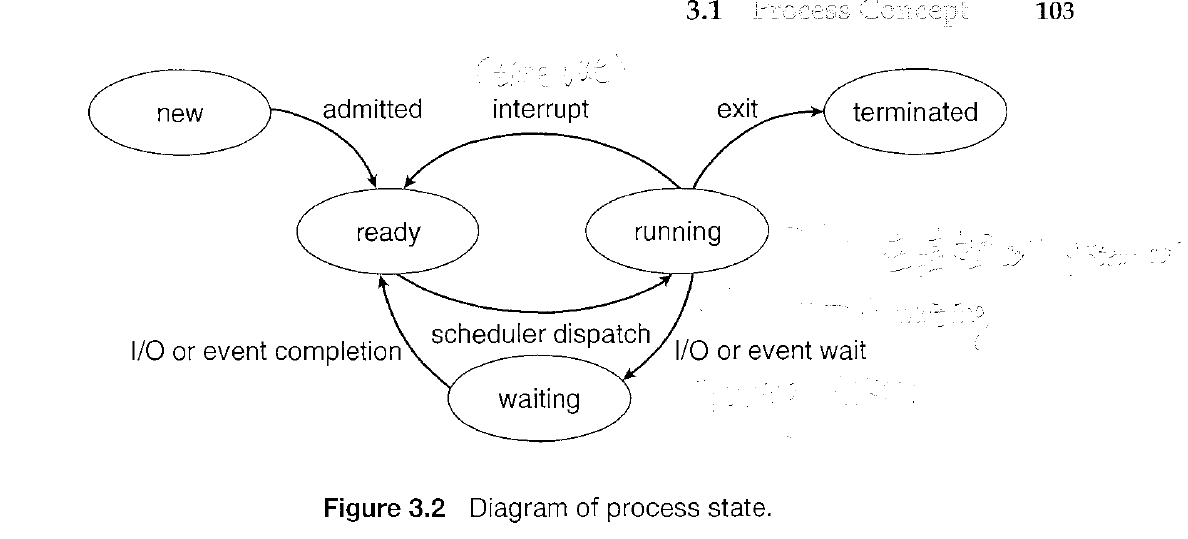
\includegraphics[scale=0.4]{process-states-silberschatz}
    \caption{Lifecycle of a process\label{pic:process-lifecycle}\cite{silberschatz2009operating}}
    %TODO own picture!
\end{figure}

The model described applies to each individual process.
For the coordination of the entirety of processes, the schedule, an operating system kernel's component is responsible.
It is a good example for the separation of mechanism and policy.
The mechanism behind is based on the \textit{multiprogramming} model as the switching of the \ac{cpu} between programs is called.
It not only allows the impression of parallelism on a single processing core, but also increases its utilization, as many processes spend a lot of time waiting for external events such as keyboard inputs\cite{tanenbaum-modern-operating-systems}.

Principally, the mechanism behind scheduling does not differ fundamentally from the treatment of an ordinary interrupt.
First, the \acf{pc} is saved prior to the new \ac{pc} is loaded from the interrupt vector and the \ac{cpu}'s registers are saved.
After a new stack was setup, the actual interrupt service runs before the scheduling policy decides which process is to run next and the selected one is started\cite{tanenbaum-modern-operating-systems}.

\subsubsection*{Process Creation}
There are several reasons why a new process should be started and scheduled at all.
The most basic one is the systems start-up.
To initialize an operating system are numerous processes created to execute parts of the system itself.
The user perceives very few of them directly, since the most of them are \textit{background processes} performing specific tasks like accepting incoming mails.
Often, long running processes without user interaction are referred as \textit{deamon processes}\cite{glatz2015betriebssysteme},~\cite{tanenbaum-modern-operating-systems}.
They are mostly generated from the \textit{init process}, the first one running and bringing up the system.
Foreground processes, the ones a user interacts with, are more often started on behalf of the user.
Besides, a process can also be started by a system service call from an existing process.
The last option, that a process is started to execute a batch job is rare today apart from scientific high performance computers\cite{tanenbaum-modern-operating-systems},~\cite{glatz2015betriebssysteme}.
%TODO graphic

Also, for the way how a new process can be started there are several options.
Using \textit{process chaining}, a running process starts an independent new one, a new \ac{pcb}, and destroys itself\cite{achilles2006betriebssysteme}.
An example is the Unix implementation of \texttt{exec()}\cite{glatz2015betriebssysteme},~\cite{tanenbaum-modern-operating-systems}.
By \textit{forking a process}, a second one that is, at least in the beginning, a copy of the original one.
Both remains exiting and share the same environment such as program code, address space and resources\cite{tanenbaum-modern-operating-systems}.
As a result, both processes have access to the exactly same resources like opened files or \ac{io} devices\cite{achilles2006betriebssysteme}.
The Unix implementation of \texttt{fork()} is an example for this way of process creation.
Process \textit{forking} and \textit{chaining} are usually used combined in Unix-like systems to create a new, independent process which is running in parallel to the first one\cite{tanenbaum-modern-operating-systems}.
In contrast, Windows offers a third way the \textit{process creation} which combines them in a single instruction to start a second, independent process (\texttt{CreateProcess()})\cite{glatz2015betriebssysteme}.

Are the newly created process and its parent share the same program code, the new one can simply inherit all needed data from its parent like it is done by \textit{process forking}\cite{achilles2006betriebssysteme}.
Since each process has its own virtual address space if not shared through inheritance, so the data cannot be copied there without further ado.
This is not only necessary for the multiprogramming model, but also a security mechanism that encapsulates and protects applications in execution against each other, called \textit{process isolation}.
Is it the case, e.g.\ for the once created via \textit{process creation}, an operating system needs a mechanism to pass data to the created process.
As a solution, a mechanism for the communication between processes with which the parent process communicated the new data to the child one via a buffer is just as conceivable as the use of initial parameters which are transmitted during the process creation, e.g.\ via a system call\cite{glatz2015betriebssysteme}.
The first option is used by the \texttt{popen()} call of Unix-like systems while the mechanism behind the \textit{\ac{ipc}} takes a major role in modern operating systems and therefore is treated in a separate section.
The second one is more often used for \textit{threads} which are the topic of the following section.

\subsubsection*{Process Termination}
Reaching the end of its lifecycle (see figure~\ref{pic:process-lifecycle}), a process terminates itself regularly and voluntary (\textit{normal exit})\cite{tanenbaum-modern-operating-systems}.
In addition, a process can terminate itself prematurely for various scenarios or be terminated by the operating system or other processes.
For example, a process may detect an internal error and voluntary terminates itself ahead of time or the operating system detects such an error and terminates the process involuntary to avoid major damage\cite{tanenbaum-modern-operating-systems}.
Besides, a process may gets involuntary terminated or killed by another process. 
Killing another process is in common a privileged task which require an authorization or extended rights\cite{tanenbaum-modern-operating-systems}.


\subsection{Threads}\label{sec:threads}

% whats a thread why threads

% \cite{mandl2014Grundkurs}: processes are expensive, threads are resource-saving -> a concurrent execution unit within a process, also named light-weight process (LWP), all threads within a process share the same addres space, the one of the process -> same process data, program code, global variables, resources -> light-weight because they share the resources
% besides the inherit context of the process (containing open files, ...) they have an own stack for local vars, own register and pc
%
% \cite{brause2017betriebssysteme}: processes needs much memory (not the address space alone but also the pcb entry) -> for a number of processes it is more than can be cached in ram -> switching processes is a heavy operating and takes a long time
% much applications do not need a completely new contest, but threads for execution within one process -> app waits for keyboard input and checks text for errors at the same time
% -> threads as solution (lwp)
%
% \cite{glatz2015betriebssysteme}: basic idea: parallel actions based on the same resources (address space, files, io devices) -> parallel actions within a process, process manages the resources and threads -> no isolation or saftely between threads -> data may get corrupted/seen by another thread in the same process
% process manages resources, thread executes the code -> each process contains at least one thread to execute code
%
%
% processes are used to group resources together, threads are the entities scheduled for the execution on the cpu
% threads: allow multiple executions to take place in the same environment. (multithreading)
%
% \cite{silberschatz2009operating}: benefits: responsiveness, resource sharing, economy (allocation memory and resources for process creation is costly), scalability (multiprocessor arch)

The current process concept, as previously introduced, provides only a single thread of execution.
However, this an issue as soon as a resource needs to be edited in parallel.
If a user edits a file for example, the process has to wait for the user's input repeatedly. 
It is nearly impossible to check this input for errors at the same time, since a second process is not allowed to access resources allocated by another process without an explicit action of programmers (like explicit \acl{ipc})\cite{tanenbaum-modern-operating-systems},~\cite{brause2017betriebssysteme}.

The \textit{thread model} should solve this issue.
Its basic idea is to equip a process with several execution threads that work on the same resources running in quasi-parallel\cite{tanenbaum-modern-operating-systems}.
This means processes only group the resources together while \textit{threads} represent the actual execution units on the \ac{cpu}\cite{tanenbaum-modern-operating-systems}.
A program is still abstracted as a process while (parallel) sequences within the program correspond to threads.
As a result, \textit{threads} can be considered as slimmed down processes sharing the same address space and physical resources.
Each thread has its own \acp{pc}, register set, stack and state, but the address space, global variables, open files and accounting information are shared\cite{tanenbaum-modern-operating-systems}.
A thread's lifecycle is equivalent to process's ones, but in contrast to them are threads not isolated and protected against each other\cite{glatz2015betriebssysteme}.
As they share the same address space, one thread can read, write or even destroy another thread's private stack\cite{tanenbaum-modern-operating-systems}.
Another issue are competing threads that try to write the same global data.
They cause a \textit{race condition} which possibly result in inconsistent or wrong data\cite{brause2017betriebssysteme}.

Nevertheless, the advantages of using \textit{threads} (multithreaded programming) predominate.
The most important one is resource sharing. 
The fact multiple threads using the same resources by default, e.g.\ files, in pseudoparallel are the biggest advantage but at the same time the biggest problem of this concept.
Threads enable responsive, interactive applications and increase the performance especially on multiprocessor architectures they can run truly parallel\cite{silberschatz2009operating}.
Another reason is an economic one.
While allocating an address space and physical resources to create a process is an expensive operation, creating a thread is not as they inherit exactly these components from their corresponding process\cite{silberschatz2009operating},~\cite{mandl2014Grundkurs}.
Threads only need to set up their own \ac{pc}, registers, stack and a state within a process. 
That's why they are also known as \acf{lwp}\cite{mandl2014Grundkurs}.

How \textit{light-weight} they actually are depends on a lot to their implementation in an operating system.
Conceivable options are thread implementation in userspace or kernel space, but also hybrid ones. 
Implementing them as user library requires an own mechanism to schedule threads within a process which is often realized as a kind of runtime environment including a \ac{tcb} (according to \ac{pcb}) for each single process\cite{mandl2014Grundkurs},~\cite{tanenbaum-modern-operating-systems}.
There is no need to invoke the operating system to switch a thread, but as a result all threads within a process block become blocked if a single one waits for a resource\cite{tanenbaum-modern-operating-systems},~\cite{brause2017betriebssysteme}. 
The operating system's schedule just do not know about the runtime environment and possible other runnable threads within a process.
The implementation in kernel space is not that light-weight, but multicore architectures benefits more from this variant.
If the operating system's kernel has the control over threads, these are managed just like processes.
Instead of one \ac{tcb} within each process, the kernel collects the \acp{tcb} for all threads in the entire system in a thread table according to the process table\cite{tanenbaum-modern-operating-systems},~\cite{mandl2014Grundkurs}.
But this also allows the kernel to recognize a blocked thread and schedule another one of the same process instead of blocking the whole process\cite{tanenbaum-modern-operating-systems}.


\subsection{Processes and Threads in Linux} 
As in the general model, a process in Linux corresponds to a program in execution.
Initially, a process contains exactly one thread of execution but further ones can be created as soon as the process has started\cite{tanenbaum-modern-operating-systems}.
Processes are organized in a tree-like structure with the so-called \textit{init} process on its top.
Starting from init, each new process to be created is split off from its parent using the \textit{fork()} system call.
Forking a process, the newly created child process inherits the whole environment of its parent including environmental variables, opened files and network connections.
Furthermore, it gets a copy of its parents address space including the data and code sections.
As both processes share the same data and resources at this time, synchronization is needed if both try to access the same one\cite{mandl2014Grundkurs}.
This issue is considered in the following section~\ref{sec:synchro}.
The distinction of parent and child is done via their \ac{pid}.
The fork call returns 0 to the child and a non-null \ac{pid} to its parent. 
Based on this, the execution paths can be splitted up\cite{tanenbaum-modern-operating-systems},~\cite{mandl2014Grundkurs}.
Even if parent and child differ only by the \ac{pid} directly after the fork, changes in the parent are not visible to the child and vice versa.
To take advantage of this fact to actually use the new created process independently of the parent, in Unix-like systems the fork call is in most cases directly followed by the call \textit{exec()}, which replaces the complete process environment with the one from another, new program.
As copying the process data is quite costly and needless if an exec follows directly, modern Linux systems use a \textit{copy-on-write} strategy for process forking.
Childs get own page tables pointing to the parent ones.
The child still can read the parent's environment data without a copy operation needed. 
Only when the child tries a write access on this data, a \textit{protection fault} is thrown and the page to modify is copied to the child process\cite{tanenbaum-modern-operating-systems}.
Such a fork is known as \textit{vfork()} and used especially in situations an \textit{exec()} follows directly to avoid the expensive and needless copy of the parent process's environment\cite{mandl2014Grundkurs}.

Within the Linux kernel, the difference between processes and threads (or heavy-weight and light-weight processes) is not as important as described in the general section about processes.
It is rather spoken of \textit{tasks}.
The reason for this is that the Linux kernel offers a possibility for a fine-granular process respectively thread creation via the \textit{clone()} call on kernel level.
In addition, Linux respects \ac{posix} threads\cite{lfd430}.
But as the clone call is a unique feature of Linux and not generally available on other Unix-like systems are application using the clone call directly not portable\cite{tanenbaum-modern-operating-systems}.

Nevertheless, \textit{clone()} is a very interesting concept in Linux.
In each case, a process or thread created with clone gets an empty private stack and executes directly a new program which is given as an argument to the call.
The decisions whether a process or a thread should be created, which resources should be shared or copied and which process is actual the parent are based on the following flags:
\begin{itemize}
    \item if \texttt{CLONE\_VM} is set, a new thread is created, if not, the call results in a new process.
    \item if \texttt{CLONE\_FS} is set, the newly created thread or process shares \textit{umask}, \textit{root} and \textit{working directories} with its parent. They are not shared at all if the flag is not set.
    \item if \texttt{CLONE\_FILES} is set, the parent shares file descriptors with its child. If not, they are copied to the child.
    \item if \texttt{CLONE\_PARENT} is set, the child's parent is the same as the calling process ones. If the flag is not set, the calling process becomes the parent\cite{tanenbaum-modern-operating-systems}.
\end{itemize}

The flags listed show only a partial amount of the possibilities \textit{clone()} offers.
A full list the glibc wrapper to the corresponding systemcall is available as a man-page using \texttt{man 2 clone}.
Both, processes (tasks) and threads based on the clone call are kernel constructs.
The \ac{posix} thread implementation on Linux internally also uses the clone call with the special flag \texttt{CLONE\_THREAD}.

In contrast to the process lifecycle presented in the generic section, Linux tasks have one extra state called \textit{zombie} which is entered on process termination until the parent process is informed about\cite{mandl2014Grundkurs}.
%TODO deamons in linux?


\subsection{Processes and Threads in Zircon}
Similar to Linux, runnable entities of the Zircon kernel are called \textit{tasks} objects.
This term includes the kernel objects \textit{jobs}, \textit{processes} and \textit{threads}.
As the whole Zircon kernel is object-based, the user interacts with kernel objects like the ones mentioned above via handles.
The Zircon documentation describes \textit{handles} as ``kernel constructs that allows user-mode programs to reference a kernel object''\cite{zircon-process}, containing the reference to this object, the corresponding rights and the user-space process bounded to.
Thus, a handle can reference each object type listed in the \textit{Zircon Kernel objects} reference\cite{zircon-objects}, including kernel objects for drivers like \textit{interrupts}, \textit{resource} objects and \textit{Log} objects.
The Zircon systemcall \texttt{zx\_status\_t zx\_task\_kill(zx\_handle\_t handle)} is such an interaction between a user application and the kernel. 
It refers to a \textit{task} object handle and thus to all objects for which \textit{task} is a generic term\cite{zircon-task}.
% All objects included in the definition of the term \textit{task} have in common that they can be suspended, resumed and killed.

\textit{Jobs} as an organizational unit are Zircon-specific and not known from the general or the Linux-specific section on processes and threads.
A \textit{job} manages a group of processes but possibly other (child) jobs, too.
According to Linux, jobs built a tree structure as every process must belong to a single job but jobs can be nested.
Except the root job, which corresponds to the init process on Linux, each one has only one parent.
A Job object consist of a reference to a single parent job, a number of child jobs and a set of member processes.
In future\footnote{Unless otherwise noted, the status of the Zircon documentation cited in this thesis corresponds to the forked and frozen source code repository on which basis the driver development takes place. See \url{https://github.com/Allegra42/zircon/blob/i2c-grove-lcd/docs/}.}, they will also contain a set of policies\cite{zircon-job}.
Jobs are used to track the privileges needed to perform kernel related operations like systemcalls but also to track and limit the consumption of basic computing resources such as memory, \ac{cpu} time or \ac{io} devices\cite{zircon-job}.
The idea behind this concept is managing applications composed of more than one process as a single entity, both from a resource and permission view as well as from lifetime control\cite{zircon-process}.

A Zircon \textit{process} itself is an instance of a program as defined in the general section about processes~\ref{sec:processes-threads}.
It consists of the program code as a set of instructions to be executed by one or more \textit{threads} and a collection of resources.
Threads are just as much a part of a process' resources as \textit{handles} and \textit{\acp{vmar}} are\cite{zircon-process}.
Strictly speaking, it is not necessary to mention \acp{vmar} as an own point.
They are kernel objects itself.
But as the documentation mentions them explicitly, they should also receive special attention in this place.
A \ac{vmar} represents a contiguous part of virtual memory address space used by the kernel as well as by the user-space. 
Each process starts an own \ac{vmar} to built up its address space.
\acp{vmar} have a hierarchical permission model, so a process with a read only address space cannot create a readable and writable one, and are randomized per default\cite{zircon-vmar}.

The lifetime of Zircon processes differs from the general but also from the Linux model.
In Zircon, a new process is created via \texttt{zx\_process\_create()} but the execution starts not before \texttt{zx\_process\_start()} is called.
Once a process started and exits its last thread, it is impossible to add a new thread.
Processes which are composed to a job are threatened as a single entity from a lifetime control's point of view.
The lifetime of Zircon processes (or jobs) ends if 
\begin{itemize}
    \item the last thread within the process or job exits or is terminated,
    \item the process or job itself calls \texttt{zx\_process\_exit()},
    \item the parent job terminates the process or
    \item the parent job is destroyed\cite{zircon-process}.
\end{itemize}

Just like known from the general section are Zircon \textit{threads} the actual runnable computation entity living within a process.
They are created within the \textit{process} context via \texttt{zx\_thread\_create()} but as it is done with Zircon processes, the actual execution is not started until \texttt{zx\_thread\_start()} \textbf{or} \texttt{zx\_process\_start()} is called.
The \texttt{main()} function or entry point of an application should be the first one started via \texttt{zx\_process\_start()}.
But returning from such an entry point does not terminate a thread's execution.
This must be done manually by voluntary calling 
\begin{itemize}
    \item \texttt{zx\_thread\_exit()},
    \item \texttt{zx\_vmar\_unmap\_handle\_close\_thread\_exit()},
    \item \texttt{zx\_futex\_wake\_handle\_close\_thread\_exit()}
\end{itemize}
on the thread itself\cite{zircon-thread}.
Even if the last handle to a thread is closed, the thread is not terminated automatically.
Instead, the thread must be killed explicitly after the handle was restored via calling \texttt{zx\_object\_get\_child()} on the parent.
On the other hand, a thread can be terminated involuntary 
\begin{itemize}
    \item if the parent process is terminated,
    \item if someone calls \texttt{zx\_task\_kill()} on the thread's handle and
    \item if an exception was generated for which is no handler or the handler terminated the thread\cite{zircon-thread}. 
\end{itemize}

In contrast to Linux threads and some library thread implementations, Zircon threads are always \textit{detached} from each other.
An operation like \texttt{join()} which waits for an undetached thread to complete and allows a clean termination is not needed in Zircon itself.
Libraries and runtime environments on top of Zircon may require such an operation to reach e.g.\ \ac{posix} compatibility\cite{zircon-thread}.


\section{Synchronization and Inter Process Communication}\label{sec:ipc-and-synchro}
% The term \ac{ipc} is not only used for pure communication between different processes but also for their synchronization\cite{glatz2015betriebssysteme}.
% The latter has already been dealt with in the previous section.
% In this one, especially the communication between different processes is to be considered.
% The one between threads of the same process has previously been discussed.
The term \acf{ipc} is not only used for the pure communication between different processes but also for the synchronization between processes, threads and data shared between them.
In this context mentioned already the previous~section~\ref{sec:threads} that the ability of threads to access shared data not only has advantages.
As they share storage, e.g.\ main memory, two threads can read and write the same value.
But what happens if both of them try to access the same, shared value?
Two threads try to read and modify a shared value are given for example.
Both read the value and calculate based on the read a new one to store. 
There is no problem as long as they just read the same value, but it occurs on updating the value.
May the first thread is scheduled first and updates the value, directly following the second one is scheduled and updates the value based on the value read before the first thread was executed.
In this case, the update of the first thread is lost. 
The data becomes inconsistent.
Such a situation is called \textit{lost update problem}\cite{glatz2015betriebssysteme}.
Unless the scheduling of the threads is predictable in each situation, it remains impossible to predict the exact outcome.
Therefore, one speaks of a \textit{race condition}\cite{tanenbaum-modern-operating-systems}.
The section~\ref{sec:synchro} deals with corresponding problems, especially for threads, and indicates ways to deal with them.
Since it is not sufficient to allow only the exchange of data respectively communication between threads of a single process, section~\ref{sec:ipc} shows mechanisms that overcome the process isolation and enable the communication between multiple ones.

\subsection{Synchronization}\label{sec:synchro}
% Already the previous section mentioned that the ability of threads to access shared data not only has advantages.
% As they share storage, e.g.\ main memory, two threads can read and write the same value.
% But what happens if both of them try to access the same, shared value?
% Two threads try to read and modify a shared value are given for example.
% Both read the value and calculate based on the read a new one to store.
% There is no problem as long as they just read the same value, but it occures on updating the value.
% May the first thread is scheduled first and updates the value, directly following the second one is scheduled and updates the value based on the value read before the first thread was executed.
% In this case, the update of the first thread is lost.
% The data becomes inconsitent.
% Such a situation is called \textit{lost update problem}\cite{glatz2015betriebssysteme}.
% Unless the scheduling of the threads is predictable in each situation, it remains impossible to predict the exact outcome.
% Therefore, one speaks of a \textit{race condition}\cite{tanenbaum-modern-operating-systems}.

In the context of this section, it should be assumed that \textit{threads} are implemented as a part of the operating system's kernel rather than based on a runtime system.
According the definition, the term \textit{thread} refers in this section both, execution threads within a single process and the ones within independent processes.
A competitive situation can occur for both variants. 
The threads of one process rather rival regarding a shared variable while the threads of different processes rather compete for resources such as a printer.

Race conditions are a topic each time several processes or threads work on the same data in any way.
This also applies to an operating system's kernel, except for non-preemptive  kernels which can guarantee that only one thread is active at a time\cite{silberschatz2009operating}.
In contrast to preemptive kernels, non-preemptive ones do not allow a thread running in kernel mode to be interrupted. 
The thread runs until it exits kernel mode, blocks or yields the control of the \ac{cpu} voluntary\cite{silberschatz2009operating}.
Only in such a case can be guaranteed that a kernel and its data structures are free of race conditions.
However, preemptive kernels are more common because they are more responsive and better suited for real-time tasks due to their interruptibility\cite{silberschatz2009operating}.
Furthermore, with today's multicore systems is it rather unlikely to fulfill the requirement of only one active thread in kernel space.

For this reason, a mechanism to prevent race conditions on both, user and kernelspace, is needed.
The basic idea behind is to exclude the chance that a thread trying to change a shared resource is interrupted by another one trying to work on the same resource\cite{tanenbaum-modern-operating-systems}.
But only certain areas in the program code are critical, the ones a shared resource is processed.
They are called \textit{critical regions} or \textit{critical section}\cite{tanenbaum-modern-operating-systems}.
Other regions do not harm if they are interrupted.
If only one thread at a time is allowed in critical sections and another one is not allowed to enter the region until the competing access is completed, this is called \textit{mutual exclusion}\cite{tanenbaum-modern-operating-systems}, \cite{glatz2015betriebssysteme}.

The easiest way to achieve \textit{mutual exclusion} is to completely disable the system's interrupts immediately after entering a critical region and re-enable them just before leaving it.
In the meantime, all incoming interrupts are collected and processed as soon as they become re-enabled\cite{achilles2006betriebssysteme}.
However, this method is not suitable for modern multicore systems since the interrupts can only be locked for the current \ac{cpu} core.
The competing thread can still modify the resource if executed on a different core.
This solution is not ideal for single core systems, too, because even the clock interrupt is disabled and with this the process scheduling.
Does the currently running thread not re-enable the interrupts, the whole system is blocked\cite{tanenbaum-modern-operating-systems}.

While there are some approaches to pure software solutions such as the algorithms of \textsc{Peterson} or \textsc{Dekker} (see \cite{tanenbaum-modern-operating-systems} or \cite{silberschatz2009operating} for further information) are hardware enabled solutions common today\cite{tanenbaum-modern-operating-systems}.
Modern multicore \acp{cpu} usually offer an instruction which is referred as \ac{tsl} or \ac{tas} in literature.
It is an atomic, not interruptible operation, usually used to modify a shared variable which controls the access to a shared memory region\cite{tanenbaum-modern-operating-systems}.
The atomicity of a \ac{tsl} instruction is in common achieved by locking the memory bus to prevent other \acp{cpu} from accessing the memory until the operation is done.
As a big advantage of this solution, the \ac{cpu} cores are not obstructed.
Common calculations are not impeded but memory accesses are prevented\cite{tanenbaum-modern-operating-systems}.
A variant is the \ac{xchg} instruction which exchanges the content of two memory locations in one atomic operation\cite{silberschatz2009operating}.

All mechanisms mentioned so far have one problem: they require busy waiting.
The thread waiting is still active and waists \ac{cpu} time.
For short waits, this is perfectly fine.  
Switching to another thread and back would be more expensive in such a situation\cite{glatz2015betriebssysteme}. 
Thus, there are locking mechanisms that implement busy waiting very efficiently, called \textit{spinlocks}\cite{tanenbaum-modern-operating-systems}.
But longer active waits are very inefficient.
In this case, it is better to use blocking waits and bring another thread in execution until the reason for the blocking is removed, e.g.\ the desired resource is freed again.

\subsubsection*{Semaphores and Mutexes}
\textsc{Dijkstra} suggested in 1965 a possibly blocking lock mechanism called \textit{semaphores} based on a \ac{cpu}'s \ac{tsl} instruction and easier to use for application developers.
A \textit{semaphore} is a new integer typ with two related operations called \textit{P} and \textit{V} in the original paper or \textit{down} and \textit{up} in some literature and implementations\cite{glatz2015betriebssysteme}.
The semaphore is initially initialized with a value greater 0, the exact one depends on a system's implementation or can be defined by a programmer.
If the \textit{P} or \textit{down} operation is executed on a semaphore, it is checked whether the value is greater than 0, decrements the counter if it is the case and continues. 
If not, the thread is put to sleep.
The operation remains unfinished until a \textit{V} or \textit{up} operation was executed and incremented the semaphores value.
One of the possibly multiple threads sleeping on a semaphore is randomly or by a certain rule chosen by the operating system and gets the clearance to complete the \textit{P} or \textit{down} operation\cite{tanenbaum-modern-operating-systems}.
For a semaphore, the fact updates on its value must be performed in an atomic operation is essential\cite{silberschatz2009operating}.
Neighter the decrementing of the value performed in the \textit{P} operation nor the incrementing in \textit{V} may be interrupted.

Semaphores are a generic approach to control access to a \textit{critical section} for a number of threads, but the often required mutual exclusion is only given if the semaphore is initialized with the value 1.
These particular case of a binary semaphore is also referred as \textit{mutex}.
A \textit{mutex} guarantees mutual exclusion for a critical section protected with its related operations as \textit{lock} (\textit{P, down}) and \textit{unlock} (\textit{V, up})\cite{tanenbaum-modern-operating-systems}.
Except for the initial value and the operation's names, mutexes do not differ from semaphores.
Just like semaphores, they can be implemented using the \ac{tsl} or \ac{xchg} instruction.

But if semaphores are actually blocking depends on the implementation.
As mentioned earlier is a blocking mechanism not always advantageous, e.g.\ for very short waits or multicore systems with real parallelism.
In these cases, its is potentially more efficient to use busy waiting with spinlocks\cite{glatz2015betriebssysteme}.

\subsubsection*{Futexes}
Another variant of semaphores is the \ac{futex}. 
It targets the issue that neighter busy waiting nor block and reschedule another thread is very efficient on modern multicore \acp{cpu}.
On a very parallel system, there are many contentions for resources which would require frequent switching of the active threads, but scheduling another thread respectively process requires as well expensive switches to the kernel\cite{tanenbaum-modern-operating-systems}.
\acp{futex} are not a pure userspace construct even if the name suggests. 
They still need a wait queue in kernel to manage the contenting threads waiting on a lock, schedule another thread (futexes are blocking by design) and putting a thread into the queue requires a system call as well.
An user library tests a lock variable using a \ac{tsl} instruction.
If the lock is already held by another thread, the library has to put the thread to the queue.
But if there is no contention is there also no need to involve the kernel\cite{tanenbaum-modern-operating-systems}.
The less actual competitive situations occur, the more efficient are futexes compared to common mutexes.
Mutexes are for example used as part of the Linux kernel. 
In this context, \textsc{Ingo Molnar} published an article\footnote{\url{https://git.kernel.org/pub/scm/linux/kernel/git/torvalds/linux.git/tree/Documentation/robust-futexes.txt}} as part of the Linux kernel documentation covering the implementation of robust futexes and its impact on the system performance.

\subsubsection*{Barriers}
So far, the synchronization of resource accesses has been discussed.
Sometimes, this is not an issue but coordinate and synchronize the sequence flow of two or more threads.
If threads within an application are divided into self-contained phases, it must be ensured that the next phase is not started until the current one has been completed by all threads involved\cite{tanenbaum-modern-operating-systems}.
The synchronization points where the threads have to wait for each other to enter the next phase are called \textit{barriers}.
An example for such a situation could be cooking.
The stoven must not be switched on until all ingredients have been purchased.
In contrast to the general implementation of barriers, a common real world stove does not block itself should this not be the case.
In most instances, barriers are alternating implemented on the basis of blocking semaphores\cite{glatz2015betriebssysteme}.
%TODO more? example for two threads (A locks B, B locks A, A unlocks B, B unlocks A)?
% glatz page 203



\subsection{Inter Process Communication}\label{sec:ipc}
While the previous section~\ref{sec:synchro} focuses on threads, the actual one explicitly deals with the communication between different processes and their synchronization.
As \ac{ipc} is a central element in operating systems, especially in microkernel architectures, which significantly influences the system's behavior and performance are design aspects and their effects an essential component to be considered.

\subsubsection{Memory Based Communication}
Since the communication of threads of one process via its shared address space is already known, it is obvious to think about a comparable technique between processes as well.
But in contrast to threads within a process, the concept of process isolation must be considered here.
As a security feature, it is not possible for processes to share their address space. 
% There are two basic ways independent processes can communicate with each other.
The basic idea to implement a corresponding idea nevertheless involves the idea of using an \textit{external shared memory region} which is requested from the operating system.
It allocated the memory and show it in the address space of both processes\cite{brause2017betriebssysteme}.
The shared memory region is the responsibility of the processes, must be managed and secured against incorrect access by themselves\cite{brause2017betriebssysteme},~\cite{glatz2015betriebssysteme}.
As known from thread communication, the advantages from this solution are the performance and transparency of raw memory access, but it also needs additional (manual) synchronization to obtain and maintain consistent data\cite{glatz2015betriebssysteme}.
Nevertheless, breaks this solution the isolation between processes. 
A variant of this idea is using \textit{files} or similar resources as a communication medium.
In this case, the process isolation remains, but manual synchronization, as described in the previous section, is still necessary\cite{brause2017betriebssysteme}.


\subsubsection{Message based communication}
Message based communication methods are more wide-spread.
In contrast to the memory based ones, the synchronization usually does not have to be done manually.
The message exchange and with it the synchronization are provides by the operating system respectively its kernel via two primitives: \textit{send()} and \textit{receive()}\cite{tanenbaum-modern-operating-systems}.

Basically, there are three types of messages:
\begin{itemize}
    \item A \textit{Message} is characterized by a delimited amount of data within a single communication.
    \item \textit{Streams} can theoretically transport an unlimited amount of data. In practice, there is a limitation not visible for the sender and the receiver.
    \item \textit{Packets} organizes the data to transport in standardized formats, the communication protocols. They allow fragmented transfer of a large quantify of data which is defragmented on receiver side. The system implementation hides this fact, so the packets itself are not visible for an application\cite{glatz2015betriebssysteme}. 
\end{itemize}

    % message passing tanenbaum
    % \cite{tanenbaum-modern-operating-systems}
    % message passing: two primitives: send/receive (rather system calls than language constructs), if no message available, receiver can block until one arrives (or return immediately with an error code)
    % issue: lost messages -> receiver send back an acknowledgement message, if sender does not receive it within a certain time, it retransmits the message -> message was received, but ack is lost -> message got retransmitted -> receiver get it twice -> need to distinct between both, e.g. via sequence numbers (same number for a resent message)
    % example: MPI (message passing interface)

Regardless of the type of message, there are two basic operations available for message-based communication: \textit{send()} and \textit{receive()}.
These operations are commonly supported by the operating system and enable not only the system-wide but also the cross-system exchange of messages and data\cite{glatz2015betriebssysteme}.
Especially the opportunity of cross-system communication offers a significant advantage over memory-based communication, as this is the foundation for network communication.
But also the synchronization between the involved processes is simplified. 
The concept of messages avoids race conditions and makes the manual use of semaphores for application developers obsolete, as the operating system realizes the transmission of the messages and their synchronization.
However, this concept is not as efficient as memory-based \ac{ipc} concepts in terms of resources consumption and performance\cite{glatz2015betriebssysteme}.


\paragraph{Synchronous and Asynchronous Communication}
One of the most basic design decisions within message-based communication is whether to send or receive messages synchronously or asynchronously.
When transmitting messages \textit{synchronously}, both sender and receiver must be ready for the exchange at the same time\cite{glatz2015betriebssysteme}.
Is this not the case for one instance of them, e.g.\ the receiver, the other one (the sender) must block until the first one, the receiver, becomes ready.
An additional, manual synchronization is not necessary.
Even if the literature does not describe a general way to transfer messages between processes, race conditions cannot occur as long as a date is only sent from a writing process to the address space of an initially reading process and can only be modified there\cite{brause2017betriebssysteme},~\cite{glatz2015betriebssysteme}.
However, within the individual processes, the synchronization corresponds to the one known from threads (see~\ref{sec:synchro}).
But the close coupling of the processes within the synchronous communication leads to the fact that the program flow of both is no longer possible independently of each other.
Accordingly, the parallelism for processes in such a relationship is also limited\cite{brause2017betriebssysteme}.

The \textit{asynchronous} approach tries to decouple this by inserting a buffer between which is also known as \textit{mailbox} or \textit{message queue}.
So sending is possible even if the receiver is not available at one moment, as long as the buffer is not completely filled.
The receiver can read equally if the sender is not ready, but the buffer still contains messages.
Even different processing speeds between the processes involved can also be compensated in this way\cite{glatz2015betriebssysteme},~\cite{brause2017betriebssysteme}.
Only if the buffer is completely filled, the sender has to be blocked and vice versa the receiver if the buffer is emptied.
But an operation only blocks when running in a \textit{blocking operation mode}.
In a \textit{non-blocking operation mode}, a call returns immediately in such a situation but reports a full respectively empty buffer which has to be handled on application level\cite{glatz2015betriebssysteme}.
\textit{Asynchronous} communication allows an independent program flow and simplifies parallelism thereby.
Nevertheless, an additional buffer with limited size is needed.
The exact one depends on the implementation.
If this buffer is filled and the receiver is blocked, the situation is the same as before with synchronous communication.
But the main problem with this approach is that it is not possible to predict how long a message transfer takes and when a response can be expected\cite{glatz2015betriebssysteme}.
The issue is to decide whether a message is lost, the communication only takes a long time or the receiving process has crashed\cite{tanenbaum-modern-operating-systems}.

\paragraph{Connection-Oriented and Connectionless Communication}
Especially when the reliability of data transmission has a great significance, a \textit{connection-oriented} approach for message-based \ac{ipc} is chosen.
This allows to guarantee the message sequence, monitor the transmission time of them and to intervene if necessary\cite{glatz2015betriebssysteme}.
Until a (logical) connection or \textit{channel} between the communication partners has been established, the initial message receiver must be unambiguously known.
As soon as this is the case, the identification is not longer of relevance.
The established channel provides a reliable end-to-end transmission which may have the following properties:
%
\begin{itemize}
    \item An \textit{unidirectional} connection allows message transfers only in one direction at a time. 
        \begin{itemize}
            \item If the roles of sender and receiver never change, one says the transmission is \textit{simplex}.
            \item If the participants alternate act as sender or receiver, the transmission is also called \textit{half duplex}.
        \end{itemize}
    \item An \textit{bidirectional} connection allows message transfers in both directions. Both participants can act as sender and receiver at the same time. The transmission is \textit{full duplex}\cite{brause2017betriebssysteme},~\cite{glatz2015betriebssysteme}.
\end{itemize}
%
If a connection is no longer needed, it must be disconnected and destroyed.
The construction and dismantling of a connection means an additional and noticeable overhead especially for small amount of data to transmit.
Is only worthwhile if the reliable transmission between designated instances is more significant as the connection costs\cite{glatz2015betriebssysteme}.
One example for connection-oriented communication is a telephone call.

But there are also good reasons for \textit{connectionless} communication.
For example if the overhead of the connection setup is too costly for little data to be transferred or rather few data is sent to a large amount of receivers.
A real world example for \textit{connectionless} communication is radio.
The order of messages cannot be guaranteed for this connection type and also the loss of them is possible, but this has no further impact on the application\cite{glatz2015betriebssysteme},~\cite{brause2017betriebssysteme}.
Nevertheless, the recipient must be addressed anew in every single message.

\paragraph{Receiver Addressing}
Message receivers respectively their message queues are commonly addressed by a symbolic name which is managed in a system-wide or cross-system directory.
When addressing them, one speaks depending on the number of receivers and the liability of the transmission of:
\begin{itemize}
    \item an \textit{unicast}, if there is a 1:1 relationship between sender and a certain receiver addressed.
    \item a \textit{multicast}, if there is a 1:m relationship between sender and a defined group of receivers addressed.
    \item an \textit{anycast}, if there is a 1:1..n relationship between sender and group of receivers. At least one recipient from the group must receive the message.
    \item a \textit{broadcast}, if there is a 1:n relationship between the sender and all detectable receivers, whether the message actually arrives does not matter\cite{glatz2015betriebssysteme}.
\end{itemize}

\paragraph{Priority}
In literature, asynchronous message-based \ac{ipc} mechanisms are usually modeled without prioritizing messages.
A buffer, message queue or mailbox that works according the \ac{fifo} principle is suitable for this purpose.
In order to enable a prioritized message exchange, it is, iter alia, conceivable to use separate buffers or queues for each priority\cite{glatz2015betriebssysteme},~\cite{tanenbaum-modern-operating-systems}.


% \subsubsection{Network Communication}
% Communication between processes is not only limited to one system but can also take place in cross-system networks.
% The implementation of them should not be further considered at this point.
% The book \textit{Computer Networks} by \textsc{Tanenbaum} and \textsc{Wetherall} is a good resource if there is interest in the topic.
% Instead, the two basic concepts for this purpose, the Berkeley-Sockets and \acp{rpc}.
%
% \paragraph{Sockets}
%
%
% % socket
% -> enable a cross-computer data exchange via data streams, takes the idea of pipelines for distributed computer systems
% -> applications use tcp/udp
% -> socket is a communication end-point, where application and transport layer matches
    % -> stream socket -> connection oriented, reliable transport e.g. tcp
    % -> datagram socket -> connectionless, unreliable transport, e.g. udp
    % -> seqpacket socket -> data set oriented, reliable transport
    % -> raw socket, unreliable transport, e.g. ip
%
% reliable means the data is faultless transported, if not, the application is informed
% unreliable -> no information
%
% connections needs the same socket type on both sides
%
%
% \paragraph{RPC}
% % rpc
% -> call distributed/remote procedures
% -> calling process : client
% -> called procedure : server procedure
% both systems implement a notification service which implements the call including parameters into a calling and a return message
%
% sequenz: -> client stub (does not fulfill action itself, just connects to rpc server, calling procedure is blocked until the call is done)
% - wrap calling parameters in rpc message (marshaling)
% - send rpc message to server
% - wait for answer
% - get answer (rpc message) -> unmarshaling -> send results to application
%

\subsection{Synchronization and IPC in Linux}
\subsubsection*{Basic Synchronization}
Modern Linux based operating systems provide a wide range of basic thread synchronization mechanism from a user's point of view.
Examples are \ac{posix} realtime semaphores, \ac{posix} mutex and System-V semaphores\cite{glatz2015betriebssysteme}.
The underlying implementation in Linux versions starting from 2.6 is based the concept of futexes to provide an efficient locking mechanism\cite{tanenbaum-modern-operating-systems}.
While in userspace the grown structure of Linux, its openness, but also standards like \ac{posix} allows finding nearly every variant of basic synchronization mechanisms, the kernel itself is much more limited.

Within the actual Linux kernel, only \textit{spinlocks} and \textit{mutexes} are available besides \textit{atomic data operations} like \texttt{atomic\_set()}, \texttt{atomic\_inc()}, \texttt{atomic\_dec()} and others\cite{achilles2006betriebssysteme}.
As mentioned in the general section~\ref{sec:synchro}, a spinlock uses busy waiting while the kernel's implementation of mutexes is a blocking one.
Both are binary semaphore versions that only differ in terms of waiting behavior\cite{linux-locking}.
Linux versions compiled for single processing core systems and without preemption support do not provide any locking mechanism at all.
It is not needed in this case.
Preemptive single core systems provide spinlocks but they only disable preemption during a critical region\cite{linux-locking}.

\subsubsection*{Signals}
\textit{Signals} are a special concept of UNIX and Unix-like operating systems, located somewhere between process synchronization and \ac{ipc}.
They are used to transmitting events or information between processes similar to hardware interrupts\cite{glatz2015betriebssysteme}.
The most known usecase of signals is to interrupt or terminate one processes from another one, but actually they are also used for signaling and handling errors, \ac{io} events or to trigger even user-defined actions\cite{achilles2006betriebssysteme}.
Signals are in common send between processes, e.g.\ to indicate illegal instructions or memory access, arithmetic errors, expiring timers and much more.
The most of them are ignorable and/or handable by the receiving process, except from the \texttt{SIGKILL} and \texttt{SIGSTOP} signals\cite{achilles2006betriebssysteme}.

Signal handlers are commonly used to grateful terminate a process or handle the indicated situation.
They provide a default behavior which can be overwritten to handle specific signals tailored to the particular process.
In this case is it convention to raise the same signal with its default action again right after the custom handling finished\cite{achilles2006betriebssysteme}.
Each Linux process is aware to receive signals, but if a signal is ignored, the result is not predictable in most cases. 

\subsubsection*{Inter Process Communication}
\paragraph{Pipes}
Pipes were one of the first \ac{ipc} mechanisms in Unix-like systems besides shared memory between threads within a process and additional memory regions shared between processes.
They provide a message-based communication mechanism using datagram-typed messages.
Pipes are also in Linux wide-spread and especially known for process chaining like it is done in the command line instruction \texttt{ps -A | sort | more}.
This instruction takes the output of the first command, \texttt{ps -A} (show all processes), and uses it as input to the second one, \texttt{sort}, which is used as input for the last one, \texttt{more}, again.
In general, pipes can provide unidirectional or bidirectional communication between processes but ordinary Linux pipes provide only a unidirectional but buffered communication between the \textit{write-end} to the \textit{read-end} of a pipe\cite{glatz2015betriebssysteme},~\cite{silberschatz2009operating}.
A bidirectional communication requires two inverse pipes\cite{silberschatz2009operating}.
As a pipe is buffered, both processes are decoupled to some degree, which is influenced by the actual buffer size, a system and architecture dependent value.
Using a pipe synchronizes the involved processes implicitly.
A reading process is blocked on an empty pipe, a writing one on a full pipe\cite{glatz2015betriebssysteme}.
Ordinary Linux pipes are not accessible by another than the creating process.
Thus, pipes are commonly used between a parent process and its childs or between childs.
The parent creates a pipe which is inherited to forked childs\cite{silberschatz2009operating}.
For further reading, \textsc{Achilles} gives a good introduction to the implementation of Linux pipes and their usage in his book\cite{achilles2006betriebssysteme}. 

\paragraph{Named Pipes (FIFOs)}
Named pipes or \acp{fifo} are an enhancement to the ordinary pipes described previous.
In contrast to them are named pipes even between unrelated processes available.
Several writers or readers on a single pipe are possible.
Indeed, named pipes are capable for a bidirectional communication in half-duplex mode, too.
But in fact, bidirectional \ac{ipc} is done via two distinct pipes\cite{silberschatz2009operating}.
Named pipes are a special type of file which can be created with a freely selectable name at any point in a filesystem.
A writing as well as a reading process can open and use a pipe by its given name just like an ordinary file or pipe\cite{glatz2015betriebssysteme}.
Once, a named pipe was created, it exists until it is explicitly deleted. 
The termination of the process which created influences the pipe just as little as a system reboot\cite{silberschatz2009operating}.
That is not the fact for ordinary pipes as they are bounded to the creating process and its childs.
Both, ordinary and named pipes are only available between processes on the same system in Linux\cite{silberschatz2009operating}. 

\paragraph{Berkeley Sockets}
While both types of pipes are bounded to a single system, a corresponding mechanism for cross-system communication respectively network communication is needed.
The best known mechanism to do this in Linux and other Unix-like systems are Berkeley sockets.
They provide cross-system communication comparable to pipes\cite{glatz2015betriebssysteme}.
Sockets are \textit{communication endpoints}, put on top of the \ac{tcp} (connection-oriented) respectively the \ac{udp} (connectionless) as a transportation layer and identified by an \ac{ip} address together with a port number\cite{silberschatz2009operating}.
This work will not examine the transportation layer and physical networking more closely.
Using \ac{tcp}, the resulting socket is called \textit{stream socket}.
The resulting communication is stream-based.
In contrast, using \ac{udp} as transportation protocol, the socket is a \textit{datagram socket}\cite{silberschatz2009operating}.
A communication between two processes is implemented using an own socket from the same type for each one, working according a client-server model.
Sockets provide a bidirectional communication between the processes owning the endpoints with the basic operations \texttt{send()} and \texttt{recv()}.
Connection-oriented sockets using \ac{tcp} are additionally in need to establish a connection and shut it down as soon as it is not longer needed\cite{glatz2015betriebssysteme}.
%TODO is this enough?


\subsection{Synchronization and IPC in Zircon}

\subsubsection*{Synchronization with Futexes}
In Zircon, all low level synchronization mechanisms are based on futexes.
High level implementations of mutexes and semaphores such as \texttt{pthread\_mutex\_t} are built on top.
Thus, normal users and user applications are rarely directly in touch with futexes\cite{zircon-concepts},~\cite{zircon-futex}.
The Zircon futex implementation is very efficient.
It does not enter the kernel space or allocate any kernel resources in the uncontested case.
In contrast to the Linux futex implementation do Zircon futex operations key off of the virtual address of a userspace pointer while Linux differentiate private futex actions from the ones shared across the address spaces of more than one process.
Futher, Zircon futex operations do not modify the futex from the kernel, such an action is not required in the current implementation\cite{zircon-futex}.

\subsubsection*{Events and Event Pairs}
Events are described as \textit{signalable event for concurrent programming}\cite{zircon-event} and \textit{user signalable kernel objects}\cite{zircon-event}.
A variant of events are event pairs.
They are described as \textit{mutually signalable linked pairs of signalable objects for concurrent programming}\cite{zircon-eventpair}.
Unfortunately, there is not any more documentation about them and their use at all, not even in Google's zircon master repository.

\subsubsection*{Signals}
Signals in Zircon are e.g.\ used for channels to indicate it contains messages to read.
They are information exposed to applications by waitable kernel objects.
Each object can expose a number of signal including generic ones for all objects but also ones that are specific to the object type such the signal described in the example above.
Signals can be observed by processes respectively applications by \texttt{zx\_object\_wait\_one()} for example.
It is possible to wait for specific signals on several objects\cite{zircon-signals}.

\subsubsection*{Inter Process Communication}
\paragraph{Shared Memory}
Zircon provides so-called \textit{\acp{vmo}} and \textit{\acp{vmar}} which represents a contiguous region of virtual memory respectively of virtual memory address space.
Both go together and are mixed up sometimes.
Generally, the term \ac{vmar} is used for any operating according to address regions, e.g.\ allocate them, map and unmap \acp{vmo} to processes, but also to protect and destroy regions\cite{zircon-vmar}.
The term \ac{vmo} is used for actions on the memory object, such as create one and read or write it\cite{zircon-vmo}.
A \ac{vmo} represents a set of physical memory pages on the one hand, but also the potential for pages on-demand via lazy creation on the other.
Such objects are available on both, kernel and user-space and can be mapped into the address spaces of multiple, distinct processes\cite{zircon-vmo},~\cite{zircon-concepts}.
\acp{vmar} in Zircon are randomized by default and additionally allows adjusting the permissions of mapped pages\cite{zircon-vmar}.
The mapped \acp{vmo} are not only directly writable and readable.
\acp{vmo} also provide an one-shot mechanism to avoid the cost of mapping them more often into address spaces than necessary.
In such a case, a \ac{vmo} is created and initially written by one process and subsequently handed over to the control of another process\cite{zircon-concepts}.
Thus, they are very suitable for efficient \ac{ipc} via shared memory.

% \cite{zircon-concepts}
% shared memory: VMOs
% - represent a set of physical memory pages or the potential for pages (lazy creation, on-demand)
% - may mapped into the address space of a process
% - permissions of mapped pages are adjustable
% - can be directly written
% -> cost of mapping them to address spaces may be avoided by one-shot operations: create vmo, write a dataset to it -> hand it over to another process to use
%
% \cite{zircon-vmo}
% - represent a contiguous region of virtual memory -> can be mapped into multiple address spaces
% - used by kernel and userspace
% - represent paged and physical memory
% - standard methods for sharing mem between processes but also between kernel and userspace available
% - basic operation directly on them are possible

\paragraph{Channels}
Channels are Zircon \ac{ipc} objects, comparable with Pipes in Linux.
But in contrast to Linux, they are bidirectional, ordered message queues with two handles, each one refers to on end of the channel.
Channels provide a datagram oriented message based communication between arbitrary and unrelated processes\cite{zircon-channel},~\cite{zircon-concepts}.
The maximum number of handles referring to a channel respectively its ends and its message size are limited.
In common, there are two steps in sending a message over a Zircon channel.
At first, a message is atomically written into the channel.
Afterwards, the ownership of all handles in the context of the message is transferred into the channel\cite{zircon-channel}.
As a result, object handles which are written into a channel are removed from the sending process.
Handles which are read from a channel become added to the receiving process.
During the transmission within the channel, the handle still exists to ensure the life of related objects\cite{zircon-concepts}.
Threads can block on a channel until messages are available.
Short reads or writes are not supported.
This means, messages read from or written to a channel must fit, or they can not been read from or written.
In contrast to pipes on Linux, Zircon channels provide a special operation called \texttt{channel\_call()} which bundles the common situation a message is sent in one direction and its response is awaited right after.
The sending process dequeues the matching response identified by its first four bytes by itself\cite{zircon-concepts},~\cite{zircon-channel}.

% \cite{zircon-concepts}
% - ipc object
% - bidirectional
% - two-ended -> two handles, one referring to each end of the object
%
% - datagram oriented
% - maximum message size and maximum number of handles
% - does not support short read/write -> either a message fits or it does not
%
% - handles written into a channel are removed from the sending process
% - handles read from a channel are added to the receiving process -> between, the handle still exists
%
% \cite{zircon-channel}
% - ordered message queue
% - bidirectional
% - a thread can block until messages are available using wait
% - channel_call -> enqueues a message in one direction, waits for response and dequeues the response -> idenetified by first 4 byte
%
% - two steps in sending a message:
    % - atomically write message data into the channel
    % - move ownership of all handles in the message into the channel
%
% - channels are not duplicateable

\paragraph{Sockets}
There are two main differences between Zircon channels and sockets.
At first, sockets offer stream-oriented message passing instead of the datagram oriented one known of channels.
Besides, sockets can not transfer object handles\cite{zircon-concepts},~\cite{zircon-socket}.
Just as channels, sockets allow a bidirection communication with two ends.
The data is written to one handle and read from the other one. 
Both ends can fulfill both jobs, but they can also been shutdown for reading or writing\cite{zircon-socket}.
Unlike channels, sockets provide short writes if the internal message buffer is almost filled and short reads if more data than available is requested\cite{zircon-concepts}.

% \cite{zircon-concepts}
% - ipc object
% - bidirectional
% - two-ended -> two handles, one referring to each end of the object
%
% - stream oriented
% - data may be written into or read out of them in units of one or more bytes
% - short writes (if the sockts buffers are full) and short reads (if more data is requested than in the buffers) are possible
%
% \cite{zircon-socket}
% - bidirection streaming ipc transport
% - can only move data, no handles
% - data is written into one end and read from the other
% - both ends are read/writable
% - ends can be shut down for writing/reading
%
% - some signals are available for socket objects

\paragraph{FIFO}
The last \ac{ipc} object Zircon provide, is a \ac{fifo}.
There is no much documentation about yet, neighter in the usual documentation version used nor in Google's master repository ones.
\acp{fifo} are described as \ac{ipc} queues with an advantage on read and write operations.
They are intended to be a top-level interface for shared memory based \ac{ipc} which enables the performance advantages over channels and sockets.
Nevertheless, are \acp{fifo} on Zircon more limited on the size of elements and buffers than the previously named mechanisms\cite{zircon-fifo}.

% \cite{zircon-fifo}
% - first in first out ipc queue
% - intented to be the control plane for shared memory transports
% - read and write operations are more efficient thant channels or sockets
% - restrictions on size of elements and buffers
%

\section{Scheduling}\label{sec:scheduling}
% Intro
The term \textit{scheduling} was already part of this work in the context of processes and threads.
It was used to describe situations in which the actual executed processes and threads must be replaced at certain intervals to provide the impression of parallelism.
In most cases, there are much more processes ready for execution than the actual number of available execution units, the \ac{cpu} cores.
Although this work assumes modern multicore \acp{cpu} and thus real parallelism, the number of processes in interactive or realtime operating systems is much higher than the number of cores, too.
A mechanism to share the resource \textit{computing time} between all processes being in need of it is required accordingly.

Scheduling is generally used as an umbrella term for the actual \textit{scheduling}, i.e.\ the planning of the process execution and allocation of resources like computing time on the basis of certain criteria, and the \textit{dispatching}, i.e.\ the mechanism which provides the assignment of a process and its data to a \ac{cpu} core and executes their exchange\cite{brause2017betriebssysteme},~\cite{mandl2014Grundkurs}.
Since the concept of scheduling is already divided into strategy (policy) and mechanism, it is obvious to do this also in the implementation.
The mechanism of the dispatcher is familiar from context switching.
Except changing the \ac{cpu}'s operating mode, pure process switching follows the same rules.
Basically scheduling can refer to processes in the whole or individual threads\cite{mandl2014Grundkurs}.
The differences and effects of both variants have already been discussed as part of the section~\ref{sec:processes-threads}.
Scheduling strategies presented as part of this section apply to both, regardless of whether they are applied on processes or threads managed by an operating system or threads managed by a runtime environment.
Thus, it is often generally referred to as job scheduling\cite{mandl2014Grundkurs}.
Furthermore, only \textit{dynamic scheduling} is considered in the following.
In contrast to \textit{static scheduling}, changing tasks, as known from interactive or dialog driven systems, can be taken into account there.
Operating systems with a fixed and static scheduling list which are setup in advanced and not changed during runtime are rare\cite{brause2017betriebssysteme}.
In addition, a distinction is made between \textit{long term scheduling} which describes the management of all tasks arriving in an operating system, especially the skillful execution of long-running jobs at times the system is not actively in use, and \textit{short term scheduling}, the strategy to assign the processes which are currently read to run to a \ac{cpu} core\cite{brause2017betriebssysteme},~\cite{mandl2014Grundkurs}.

\subsubsection*{Scheduling goals}
Having the common case that more processes or, more generally spoken, jobs are ready to be executed, there is a need of a policy to find the next one to run.
Such a strategy is influenced by various design goals, depending on the operating system's type, its purpose and the actual application\cite{mandl2014Grundkurs}.
The goals which can be included in an individual strategy are as follows:
\begin{itemize}
    \item \textit{Fairness}, i.e.\ a minimum computing time is guaranteed for each job and no one should be preferred if not explicitly part of the strategy.
    \item The \textit{\ac{cpu} utilization} should generally as high as possible. It is the most limited resource in a computing system.
    \item \textit{Minimize response times} is especially important in interactive systems as a delayed reaction to a user input is more noticeable than a longer runtime of an already long-running background job.
    \item \textit{Minimize wait times} could also be an interest. But this fact depends not only on a scheduling strategy and the related resource synchronization but also on \ac{io} operations are not directly influenced by a job scheduler. 
    \item \textit{Maximize throughput} refers to the number of settled jobs per time.
    \item \textit{Minimize the turnaround time}, i.e.\ the complete time a job needs for its execution. As with the related point ``minimize wait times'', a scheduling strategy only impacts the time in a waiting queue.
    \item A \textit{Predictable process execution} is especially a requirement for the use in realtime operating systems\cite{mandl2014Grundkurs},~\cite{brause2017betriebssysteme}. 
\end{itemize}
But there is no single scheduling strategy that fits all situations and goals equally well.
In some cases, the goals named above even contradict each other.
However, the decoupling of mechanism and policy enables the user to change the latter one according the current needs and interests\cite{brause2017betriebssysteme}.

\subsubsection*{Scheduling policies}
One of the most important questions in the selection of a suitable scheduling strategy is whether it should be preemptive or not.
This term was also already marginally mentioned in the context of process and thread synchronization (see section~\ref{sec:processes-threads}).
The focus there was rather on the impact the interruptibility of a process or thread has on itself and shared resources.
In the context of job scheduling, a non-preemptive job implies the job runs until it voluntary hands over the control back to the system, e.g.\ because it is waiting for a resource or an event or it reaches its completion\cite{mandl2014Grundkurs}.
Depending on the exact policy, a high maximum computation time is often given nevertheless in such a case.
It prevents faulty or malicious processes from blocking an entire system\cite{achilles2006betriebssysteme}.
Even on modern multicore \acp{cpu} is a pure non-preemptive scheduling strategy rather not suitable for interactive, multiuser and realtime operating systems, but for batch jobs.
For these systems, a preemptive scheduling strategy with generally interruptible jobs is more appropriated.
The whole available computing time is sliced down into equal sized time slots which are assigned to the jobs.
If a job does not finish within such a slot, it needs to be rescheduled according a certain policy\cite{brause2017betriebssysteme}.
This makes such a system much more responsible.

Whether a scheduling policy should be aware to prioritized jobs follows directly after.
There are a lot of reasons to give priority to certain jobs, e.g.\ to create the impression of a notably reactive system by prioritize \ac{ui} related jobs or to ensure the fastest possible processing of a security-critical task in a realtime system\cite{mandl2014Grundkurs}.
In general, prioritized jobs are available on both, preemptive and non-preemptive policies\cite{brause2017betriebssysteme}.

The intention of this work is not to provide a complete enumeration of scheduling policies but a selection of relevant ones with respect to Linux and Zircon.
As a consequence, preemptive strategies for interactive multiuser and realtime systems are considered in particular.
More complete considerations are available in the books of \textsc{Brause}\cite{brause2017betriebssysteme},~\textsc{Mandl}\cite{mandl2014Grundkurs}, \textsc{Achilles}\cite{achilles2006betriebssysteme} and others.
For the introduction to scheduling strategies within this work, the individual ones are examined on basis of a single \ac{cpu} core.
In fact do modern multicore processing systems using \ac{smp} manage an own job scheduling for each core separately.
As a result, competing situations for processes and threads such as discussed in the previous section~\ref{sec:synchro} arise again.
An optimal scheduling strategy for multicore systems should therefore also take the required resources into account to avoid unnecessary blocking or context changes\cite{brause2017betriebssysteme}.
A global component named \textit{load balancer} can step in if the load on an individual core is much higher as the average\cite{achilles2006betriebssysteme}.

\paragraph{Round Robin}
\acused{rr}(\acs{rr}) is intended for the use in interactive multiuser systems.
It is an enhancement of the so-called \textit{\ac{fcfs}} strategy used in batch-oriented systems. 
\ac{rr} is applied for non-priorizing preemptive timesharing systems instead\cite{achilles2006betriebssysteme}.
All reaching jobs are put into a \ac{fifo} based queue.
The first one which was putted in is also the first one how gets assigned to a \ac{cpu} core from the scheduler.
In contrast to \ac{fcfs} as a non-preemptive strategy for batch jobs, the maximum time a job is allowed to use the resource \ac{cpu} is limited.
Does a running job not voluntary release the \ac{cpu} within its time slice, an interrupt to cut it off is triggered.
The job loses its \ac{cpu} core which becomes reassigned to the next job in the queue.
If the replaced job was not finished yet, it is enqueued again\cite{achilles2006betriebssysteme},~\cite{mandl2014Grundkurs}.
The size of the time slice, also called \textit{quantum}, is the same for each process, but the difficulty in this strategy is determination of its effective size\cite{brause2017betriebssysteme}.
Is the slice too small becomes the overhead caused by switching the process contexts superior, is its size chosen too long, the resulting strategy evokes on \ac{fcfs} more likely.
The calculation of the next job to schedule is very cheap, using \ac{rr} as a strategy\cite{brause2017betriebssysteme}.

\paragraph{Dynamic Priority Round Robin}
\acused{dprr}(\ac{dprr}) is a priority aware modification of the usual \ac{rr} scheduling strategy.
The only point that differs is an additional queue in front of the known one.
Each job arrives in the first queue with a priority and stay there until this value reaches a certain threshold.
The priority value of each job in the preceding queue is increased after a time slices is finished.
As a result a job with the priority 8 is executed prior to one with a priority of 4, even if it arrived shortly after the lower prioritized one.
The subsequent \ac{rr} strategy is not touched at all to add priority support, but the management of the additional queue requires little more management effort\cite{brause2017betriebssysteme}.

\paragraph{Shortest Remaining Time First}
\acused{srtf}(\ac{srtf}) is an algorithm for preemptive scheduling with time slices, too.
The decision for the next job is, as described by the name, made based on the shortest remaining computing time needed.
As a result, each time a slice ends and a new job needs to be assigned to a \ac{cpu} core, the remaining time for each upcoming job must be recalculated. 
Thus, the selection of the succeeding job is quite complex every time\cite{brause2017betriebssysteme},~\cite{glatz2015betriebssysteme}.

\paragraph{Multilevel Scheduling}
is a strategy to schedule various types of jobs with different importance.
The jobs are often split up into \textit{system processes} with the highest priority, followed by \textit{interactive jobs} and \textit{general jobs}. 
The lowest priority is given to \ac{cpu}-intensive and long-running \textit{batch jobs}\cite{brause2017betriebssysteme},~\cite{mandl2014Grundkurs}.
The idea for the multilevel scheduling algorithm is to hold a distinct queue for each priority level available.
Jobs in the queue with the highest priority become processed first. 
The ones in next lower priority are not touched until the higher ones are emptied.
As a consequence are situations possible where low priority processes never become scheduled.
One speaks of \textit{starvation}\cite{glatz2015betriebssysteme}.
Multilevel scheduling also allows some variants.
The actual scheduling strategy for each queue itself is variable.
\ac{rr} can be used to provide a fair scheduling between all jobs on a single priority level.
For realtime systems with one or just a few jobs in the highest level, \textit{fcfs} could be more appropriated in certain cases.
Generally is an additional reassignment of the \ac{cpu} core as soon as a high prioritized job enters its queue reasonable in realtime system using multilevel scheduling as a strategy\cite{glatz2015betriebssysteme}.

\paragraph{Fair Share Scheduling}
is a strategy to guarantee the same share of the \ac{cpu} to each single job.
Having \textit{n} jobs in the whole system, each one gets a \textit{1/n} share of the whole computing time allocated.
As a result, the computing time used so far must be tracked along with each job.
This time is compared with the actual overall time the \ac{cpu} worked.
The decision which job is assigned to the \ac{cpu} next is made on basis of the worst ratio between already consumed computing time and the overall available one.
A job scheduled according this strategy is allowed to stay active until the worst ratio is calculated for another one\cite{mandl2014Grundkurs}.

\paragraph{Earliest Deadline First} \cite{mandl2014Grundkurs}, \cite{brause2017betriebssysteme}
\acused{edf}(\ac{edf})is a realtime scheduling strategy.
Since certain critical tasks have to be completed at a given time to avoid more or less serious consequences, this algorithm uses this deadlines to decide on their basis which job must be executed next.
The strategy itself is rather complex but useless in situations where several critical jobs must be completed at the same time\cite{mandl2014Grundkurs},~\cite{brause2017betriebssysteme}.
Nevertheless, is \ac{edf} a common algorithm for hard realtime systems and an ideal strategy on single core systems with up to 100\% \ac{cpu} utilization\cite{brause2017betriebssysteme}.


\subsubsection*{Priority Inversion}\label{sec:priority-inversion}
Using locking mechanisms like semaphores respectively mutexes may lead to dangerous behavior in context of priority based scheduling.
For a basic example are two jobs, H (high priority) and L (low priority) are given.
Both jobs want to use the same resource.
The H job is scheduled as soon as it enters the \textit{ready} state.
The problem arises if the L job starts first while H is waiting for e.g.\ another resource.
L enters the critical section and occupies the contested resource.
Just in this situation, the H job becomes ready and is scheduled according to the priority based policy.
If H is busy waiting for the resource, L is never rescheduled, can not end its critical section and free the resource\cite{tanenbaum-modern-operating-systems}.
Both jobs are blocking each other, they are in a \textit{deadlock}\cite{glatz2015betriebssysteme}.
If H blocks and hands over to L again, the priorities got inverted.
A lower prioritized job runned before one with a high priority.
Such a situation is referred as \textit{priority inversion}\cite{tanenbaum-modern-operating-systems}.
The situation described here is only dangerous if the H job misses a critical deadline, but there is a very similar and serious real world example of the mars spacecraft \textit{Pathfinder}.
It also uses priority based scheduling with three jobs, H (high priority), M (medium priority, long runtime) and L (low priority).
Just as explained for the situation above, the H job becomes waiting for a resource held by the L job. 
When H blocked, the M job was scheduled and had to finished until the L job had the chance to free the resource needed by H.
But the high prioritized task of H was to reset a watchdog to prevent a system reset accompanied by the loss of data\cite{glatz2015betriebssysteme},~\cite{silberschatz2009operating}.
A more detailed description of the situation is given by \textsc{Silberschatz} in \cite{silberschatz2009operating}.

The most common technique to prevent dangerous \textit{priority inversion} is \textit{priority inheritance}, a special property of semaphores which needs to be implemented within the operating system.
If a higher prioritized process or thread is waiting for a resource occupied by a less prioritized, the priority of the second job will be raised to the one of the higher prioritized.
This ensures that the actual low prior job frees the resource as soon as possible and the truly high prioritized task can run next.
The original priority becomes restored, once the resource has been freed\cite{glatz2015betriebssysteme}.

An alternative mechanism that can act without operating system support is \textit{priority ceiling}.
Whenever a process locks a semaphore or mutex, its priority is raised to a higher level than any other process may waiting for the resource.
As soon as the semaphore respectively mutex is unlocked, the former priority is restored\cite{glatz2015betriebssysteme}.

 
\subsection{Scheduling in Linux}
As usual, modern Linux systems offer various opportunities to adjust even scheduling to the needs of its intended application.
While code running in user space may be preempted at any time, common modern Linux kernels itself can be compiled in tree variants:
\begin{itemize}
    \item As a no-forced preemption version, suitable for the use in servers.
    \item With voluntary kernel preemption for the use in desktop systems and
    \item as a fully preemptive kernel for desktop systems with low latency requirements\cite{lfd430},~\footnote{See also ``\texttt{man 7 sched}'' on Linux systems as an additional source for this section.}.
\end{itemize}
Older kernels before version 2.6.23 were not preemptive at all.
They were only disturbed by explicit or implicit sleep requests, e.g.\ if a required resource was not available, or, if enabled, on interrupts.
After the disruption, the previous task was resumed on the \ac{cpu} core.

Back on modern kernel versions, one task can not interrupt another on by itself.
As scheduling in Linux is based on time slices, is it the mission of the scheduler to assign another job to a \ac{cpu} core as soon as a slice ends.
Summarized, a job scheduled in Linux is allowed to run until
\begin{itemize}
    \item it needs to wait for a resource to be freed or a system event to complete,
    \item it reaches the end of its lifetime and exits,
    \item its time slice expires,
    \item the scheduler becomes invoked and finds another job that has to be scheduled according the current policy\cite{lfd430}.
\end{itemize}
Linux uses one scheduler per \ac{cpu} core and a global load balancer to move jobs between them, just as named in the general section.
However, both try to schedule a job on the same \ac{cpu} to minimize cache thrashing\cite{lfd430}.

Before kernel version 2.6.23, the default scheduler in Linux was named \textit{O(1)} scheduler. 
It is named after the \textit{Big-O notation} of its algorithm which classifies the runtime or memory requirements of algorithms according its inputs.
This means in case of the O(1) scheduler that the time it needs to make the decision which task is to be scheduled next is independent of the number of tasks in the system at all.
It was using a priority ordered queue for each \ac{cpu} core\cite{lfd430}.
Since kernel 2.6.23, the \ac{cfs} became the new default scheduler.
It is a fair share scheduler, similar to the strategy described in the general section.
The decision which task must be scheduled next is made on the basis of the amount of time a task has been waiting to run, divided by the number of running tasks.
The resulting time of each task is compared with the actual time received so far.
The one with the worst ratio is selected.
Thus, the finding a decision is rather complex in this strategy\cite{lfd430}.

Linux' origin is an interactive operating system kernel, but there was the desire to use it in realtime environments as well. 
For this use, the Linux kernels needed lower latencies, other preemption methods and realtime capable schedulers.
As the needed changes affect wide parts of the kernel were they initially developed as a patch set called \textit{rt\_preempt}.
They include amongst others:
\begin{itemize}
    \item Replacing spinlocks with preemptive \textit{rtmutexes} in the whole kernel.
    \item Implementing priority inheritance for locking mechanisms.
    \item Replace common interrupt handlers with preemptive kernel thread so that they can be scheduled and sleep\cite{lfd430}.
\end{itemize}

The scheduling in Linux is very finely granular adjustable to the system and its applications needs.
It is not only possible to select the grade of preemptibility and make it aware for realtime tasks, but also to set a scheduling policy for each single thread.
Three normal and three realtime policies are available for this purpose.
The normal ones are:
\begin{itemize}
    \item \texttt{SCHED\_OTHER} respectively \texttt{SCHED\_NORMAL}, as it is called within the kernel, which describes the default timesharing scheduling with a static priority level.
    \item \texttt{SCHED\_BATCH} which is used to schedule \ac{cpu}-intensive and non-interactive tasks. It has to be used with the static priority 0.
    \item \texttt{SCHED\_IDLE} which is used for tasks with a very low priority, even lower than batch jobs.
\end{itemize}
For realtime tasks, Linux provides:
\begin{itemize}
    \item \texttt{SCHED\_FIFO}, a \acl{fifo} policy just as described in the general section. It can be used with static priories greater 0. A runnable thread using this policy will immediately preempt any running task using the normal policies mentioned above.
    \item \texttt{SCHED\_RR} just as mentioned in the general section is \acl{rr} even in Linux a time slicing version of the \ac{fifo} policy.
    \item \texttt{SCHED\_DEADLINE} is the latest scheduling policy in Linux. It is available since version 3.14 and provides a variant of the \acl{edf} policy mentioned in the general section combined with the \ac{cbs} policy.
    \ac{edf} is used for the actual deadline scheduling while \ac{cbs} guarantees non-interferences between threads.
    This strategy targets hard realtime requirements. Thread scheduled with it are the ones with the highest priority which can be controlled by a user.
\end{itemize}
A much more detailed explanation of thread specific scheduling policies and their use via \texttt{sched()} is given as part of the man-pages project using the command \texttt{man 7 sched} on a Linux system\footnote{The man-pages version used is \textit{2019-03-06} on a kernel in version 5.0.2.}.  


\subsection{Scheduling in Zircon}
The Zircon scheduler was developed out of Little Kernel's one and provide just a minimal realtime aware scheduling mechanism instead of the variety of possibilities known from Linux.
But the basic mechanism behind is also already known.
Zircon scheduling is a kind of multi-level scheduling with time slicing as stated in the general section.
The scheduling is done for each \ac{cpu} core at its own and each core has its very own set of queues.
As Zircon supports 32 priority levels right now, this makes 32 \ac{fifo} queues per core\cite{zircon-scheduling}.
Each job gets the same time slice, if it is not finished with its work, it is enqueued again.
The scheduler starts with the queue with the highest priority and executes the jobs for the maximum time of a time slice.
Only when this queue is empty, the next one is considered.
If a job blocks, it is completely removed from the \ac{cpu}'s queue and added to a distinct waiting queue.
The stays there until the required resource becomes available and thus its status changes to runnable again.
The job is put back to ,whenever possible the previous \ac{cpu} core's, queue with the right prioity.
Was the job blocked before its time slice was finished, it becomes rewarded by being inserted at the front of the queue to resume as soon as possible\cite{zircon-scheduling}.

The priority of jobs in Zircon is determined on the basis of three criteria:
\begin{itemize}
    \item A base priority from 0 to 31.
    \item A priority boost. 
        \begin{itemize}
            \item A job is rewarded with an one level upgrade when it unblocks after waiting for a resource or sleeping. 
            \item A job is penalized with an one level downgrade if it voluntary give up the control. The minimum priority value in this situation is 0.
            \item A job is penalized with an one level downgrade if it is preempted after using up its entire time slice. In this situation, the priority value may become negative.
        \end{itemize}
    \item Priority inheritance is a special criteria. If a job controls a resource which is needed by one with a higher priority, the job's priority is temporary boosted up to the priority level of the other job to prevent priority inversion (see~\ref{sec:priority-inversion}). 
\end{itemize}
As a result, the effective priority is either calculated from the base value in combination with the boost or it is the inherit one\cite{zircon-scheduling}.
This policy is designed for an interactive system.
Rewarding short and non-\ac{cpu} intensive jobs affects most of all \ac{ui} related tasks which are often blocked by waiting for user interaction, while \ac{cpu} intensive background tasks are penalized for using the whole time slice and hindering the ability to react.

Zircon is per design capable for realtime tasks.
Within the scheduler is it considered by a special flag for them: \texttt{THREAD\_FLAG\_REAL\_TIME}.
Such a job is allowed to run within its priority level without being preempted until it blocks, yields or is manually rescheduled\cite{zircon-scheduling}.

A special role belongs to the \textit{idle thread}.
It lives besides the normal \ac{fifo} queues and is runned by the scheduler if there are not any other jobs ready to be assigned.
The purpose of the idle thread is to keep track of idle times, but some platform implementions may use it to implement a low power consumption wait mode\cite{zircon-scheduling}.\\
\\
At the time of writing, an additional \ac{cfs} is in work.
Its \ac{api} is compatible to the one Linux uses.
Is it not merged into the standalone Zircon repository yet, but to the development master branch of the Zircon kernel within Fuchsia.
Further information is available in the according documentation within this repository\footnote{Zircon Fair Scheduler, visited on 11.04.2019 \url{https://fuchsia.googlesource.com/fuchsia/+/refs/heads/master/zircon/docs/fair_scheduler.md}}.


\section{Memory Management}\label{sec:memory-management}
Memory management is an essential part within an operating system.
Without going into detail, some terms and principles belonging to this topic were already part of previous sections.
For example, the topics \textit{process isolation} or \textit{\ac{ipc} via shared memory} involved sophisticated concepts for the use of the main memory in particular.
The concepts of \textit{virtual memory} and private \textit{address spaces} had a special significance in this context.
Thus, this section will focus on them.

The reason for the use of such sophisticated memory management mechanisms over direct memory allocation is motivated by the need for process isolation, shared memory and similar approaches but also by the nature of a computer's memory.
In common, the memory is a hierarchical system with \ac{cpu} registers at its top.
Registers are implemented in the same technology as the \ac{cpu} itself. 
As a result, they are very limited and expensive but also very fast.
The next layer are caches.
Current systems use a hierarchical cache system itself.
The topmost layer is nearly equivalent to registers in terms of access time and costs, and thus, very small.
After two to four cache levels follows by main memory or \ac{ram}.
If it is spoken about memory within this work, the main memory is meant in the majority of cases.
In common, the main memory is implemented as \textit{Dynamic} \ac{ram}.
Accessing the main memory is 10 to 50 times slower than accessing caches, but the capacity is significantly larger (e.g. Intel Core i7-7820HQ; L1 caches are divided into data and instruction caches with 32 kilobyte each, while the total main memory installed is 16 gigabyte\footnote{Benchmarks from an Intel Core i7, 7th Generation.}\cite{mandl2014Grundkurs}.
The data of running processes and the system itself is generally held in the main memory.
The last kind of memory which is important as a part of this thesis are common hard drives and newer \acp{ssd}, used for files, not running applications and miscellaneous other data.

As a result of this hierarchy, there is often not enough space, even not in the main memory, to store the data of all running applications. 
But there is a desire for allowing processes to use more memory than physically available and for a unified contiguous view of the memory area of each process together with the needs of processes, i.e.\ the isolation between the address spaces of distinct processes but also a way to share memory for \ac{ipc} (see~\ref{sec:processes} for the details)\cite{mandl2014Grundkurs},~\cite{brause2017betriebssysteme}.
A pure static and direct memory management would not be sufficient for these purposes.
In current systems, this is mostly realized by using the mechanisms of \textit{address spaces} and \textit{virtual memory}, which already have been mentioned several times.
% The following sections explain what this implies.


\subsection{Address Space}
The term \textit{address space} covers the summary of all possible memory addresses within the main memory from 0 to $2^{32}-1$ on a 32-bit system or $2^{64}-1$ on a 64-bit one. 
The address space is divided into reserved parts for the system, applications and others.
How this division is done is defined by the operating system in an \textit{address space layout}\cite{mandl2014Grundkurs}.
Distinct parts within this layout are protected against each other, especially the system kernel itself\cite{brause2017betriebssysteme}.
But the layout distinction does not provide process isolation. 
The system is indeed divided from application processes using such a layout, however those are not separated from each other within their sections\cite{mandl2014Grundkurs}.

The term \textit{address space} is used for the memory region of applications, through, which is effectively located within the main memory's address space.
Their intern layout is specified by the compiler or a runtime based on language conventions or standards.
A C application for example, is divided into different sections like the program code itself, constants, static variables and initialized data, not initialized data, and dynamic sections for heap (data which is allocated at runtime) and stack\cite{mandl2014Grundkurs}.

However, the pure implementation of address spaces does not yet solve all the needs named above.
Although the address space at its whole is now subdivided into various regions, it is not ensured that the address space of a process within is always contiguous.
From a technical point of view, this is not always possible because the size of process address spaces differs and as a result, gaps which have to be filled as well arise\cite{mandl2014Grundkurs}.
Furthermore, data should be aligned to addresses which are divisible by four to make accessing main memory from the \ac{cpu} more efficient\cite{mandl2014Grundkurs},~\cite{brause2017betriebssysteme}.
% \cite{mandl2014Grundkurs}
% - definition address space -> summary of all possible addresses 0 to 2^32 -1 for 4GB
% - layout is defined for each operating system within a address space layout
    % - reserved parts for applications, \ldots
    % - size of a machine word -> 32/64 bit depending on the processor (or may less)
    % -> alignment to addresses which are divideble by 4 -> faster access
    % -> byte ordering
%
% - address space of programs is specified by the compiler/runtime according to conventions
    % -> they have different subspaces within their address space example for C/C++:
        % - program code
        % - constants, initialized data, static variable
        % - not initialized data (static vars too)
        % - dynamically section for runtime allocated data -> heap
        % - dynamically section for stack
%
% \cite{brause2017betriebssysteme}
% memory protection
 
\subsection{Virtual Memory}
The abstraction needed to reach the named requirements for the physical main memory is called \textit{virtual memory} or \textit{virtual address space}.
Its basic idea is to provide abstracted, contiguous views on the actual memory to processes, which was one of the goals.
A process respectively a programmer only see a contiguous memory region starting with the address 0 but not the actual fragmentated main memory used by various processes from distinct users\cite{mandl2014Grundkurs},~\cite{brause2017betriebssysteme}.
Such a virtual view to the actual main memory also enables pretending to a program that more memory is available than is actually present.
Since the entire memory region of a program is rarely needed in main memory at a time, the concept of virtual memory together with a sophisticated mechanism to load certain memory regions from disk which enables the execution of processes, even if they can not be completely loaded into the main memory.
The operating system holds needed data in the main memory while the others are stored in hard drives.
As a result, the overall memory consumption may become greater than the physical available main memory and virtual memory is not neccessarly mapped to physical memory\cite{mandl2014Grundkurs}.
An operating system unit called \textit{memory manager} virtualizes each process for itself.
Virtual memory is only logical until the memory manager maps it to physical available one during runtime.
The purpose of this unit is, besides the already mentioned, implementing
\begin{itemize}
    \item a \textit{fetching policy}, which describes a strategy to ensure a certain memory region is present in the main memory when needed,
    \item a \textit{placement policy}, which manages where newly added regions are placed within the memory,
    \item a \textit{replacement policy}, i.e.\ the strategy that comes in when there is no more free memory available and data must be removed to load the current needed ones, and
    \item a \textit{cleaning policy} trying to keep some main memory free at any time\cite{mandl2014Grundkurs}.
\end{itemize}
% Strategies used within the memory management take advantage from the so-called \textit{locality effects}.
% The two most important ones are the \textit{temporal locality} and the \textit{spartial} or \textit{memory locality}.
% They state that memory regions that were often needed in a temporal proximity in the past will continue to be needed together with a high probability in the future, respectively that virtual memory regions located close to each other are often used together\cite{mandl2014Grundkurs},~\cite{brause2017betriebssysteme}.
%
For the use within the memory management and the actual implementation of virtual memory are virtual as well as physical main memory regions divided into fixed size blocks.
The blocks in the virtual address space are referred as \textit{pages} while the ones within the physical address space are named \textit{page frames}.
Size and location from virtual pages and physically available page frames differ from each other. 
The addresses of the virtual pages are managed in so-called \textit{page tables}.
One distinct page table represents a program which is available in the main memory\cite{brause2017betriebssysteme}.
A physically available page frame can be mapped into several virtual page tables.
Shared libraries and shared memory \ac{ipc} mechanisms are implemented in this way\cite{brause2017betriebssysteme}.

Pages, respectively page frames, represent the memory blocks which are transported between hard drives and the main memory by the \textit{memory manager}.
The policies implemented the memory management take advantage from sophisticated concepts like \textit{demand paging}, i.e.\ a page is only loaded if there is a need for, and \textit{prepaging} with use of the so-called \textit{locality effects}.
The two most important ones are the \textit{temporal locality} and the \textit{spartial} or \textit{memory locality}.
They state that pages which were often needed in a temporal proximity in the past will continue to be needed together with a high probability in the future, respectively that virtual pages located close to each other are often used together.
In accordance, the memory manager tries to load pages which are needed with a high probability in near future in advance\cite{mandl2014Grundkurs},~\cite{brause2017betriebssysteme}.

Above all, virtual memory enables the sophisticated memory management requirements needed for a efficient and secure operating system with process isolation, shared memory and a contiguous view to a program's address space for example. 
Memory protection mechanisms like process isolation and access rights to a process's address space are implemented based on virtual memory, too (refer to \textsc{Brause}\cite{brause2017betriebssysteme} for more details).
But thus, a translation between virtual addresses and the physical equivalents which considers the fact that a physical memory region may be mapped into several virtual address spaces, is needed. 
To speed up this costly translations, current application-oriented \acp{cpu} are supported by two on-chip hardware mechanisms, the \acf{mmu} and the \acf{tlb}.

The \ac{mmu} is a part of the processor itself and responsible to map virtual addresses to physical ones. 
Thus, accessing the raw main memory and regions with a special meaning is in common a privileged action done within the operating system kernel. 
The \ac{cpu} sends a virtual address to the \ac{mmu} which calculates the physical one according a defined algorithm and sends the result via the address bus to the main memory.
If a needed page is not available there, the \ac{mmu} raises a special interrupt named \textit{page fault}.
It interrupts the running process so the \ac{cpu} can try to fetch the needed address from disk.
Even if only a single address is missing, the memory manager always loads whole pages to the main memory.
If the virtual memory address as a resource is available, the interrupted process is rescheduled according the currently used policy\cite{mandl2014Grundkurs}.

The \ac{tlb} works together with the \ac{mmu}.
It is an additional fast cache to speed up the assignment between virtual and physical memory addresses. 
As described previously is accessing a cache still considerably faster than accessing the main memory itself.
Similar to common L1 and L2 \ac{cpu} caches is there an own \ac{tlb} per \ac{cpu}.
If the needed address translation is already stored in the \ac{tlb}, no further access to the main memory is needed, if not must the \ac{mmu} be invoked.
Just like caches and the main memory, a replacement strategy for the \ac{tlb} is needed to ensure its efficient use.
A more detailed introduction to these hardware support mechanisms and related strategies can be consulted at \textsc{Mandl}\cite{mandl2014Grundkurs} or \textsc{Brause}\cite{brause2017betriebssysteme}.

 
\subsection{Memory Management in Linux}
%     Linux Concept -> LFD430 pic
Linux also uses a virtual memory system, on modern \ac{mmu}-enabled \acp{cpu}, but there is also a Linux kernel variant for \ac{mmu}-less architectures used for very small embedded systems, called \textit{uCLinux}.
While a usual Linux kernel with virtual memory system needs an address translation uses \textit{uCLinux} raw physical memory addresses without further protection or other sophisticated mechanisms.
But more common and focused in this work is the use of virtual memory enabled systems\cite{lfd430}.
In general is (virtual) memory management in Linux a very complex and highly architectural dependent matter.
As \textit{32-bit x86} was the most common architecture for a long time, it is often used to describe the mechanisms, but it is also very specific in a way that even the memory management for \textit{64-bit x86} architectures differs a lot.
Nevertheless, this work focuses on \textit{32-bit x86} due to the spread of the correspond terms and mentions important differences in 64-bit x86 and ARM architectures.

The Linux virtual memory management mechanism divides the available memory in various different sections.
The most basic and wide-spread terms in this context are \textit{high memory} and \textit{low memory}.
Both do only matter on 32-bit systems.
There is no such division in 64-bit systems at all.
And in fact, the meaning of the terms is not complicated.
The whole available address space in Linux is divided into virtual kernel and user addresses.
\textit{Low memory} is a term for a physical memory region in the main memory, which corresponds to the high virtual addresses used for the kernel. 
Kernel virtual addresses differ from common virtual addresses as further described in the next section.
\textit{High memory} describes the higher physical memory addresses which maps to the virtual addresses used within user applications.
As described in the general section, Linux provides an own protected address space with virtual addresses for each process, too, which are generally mapped into high memory\cite{lfd430}.
Figure~\ref{pic:high-low-mem} illustrates the context.

\begin{figure} [ht]
	\centering
	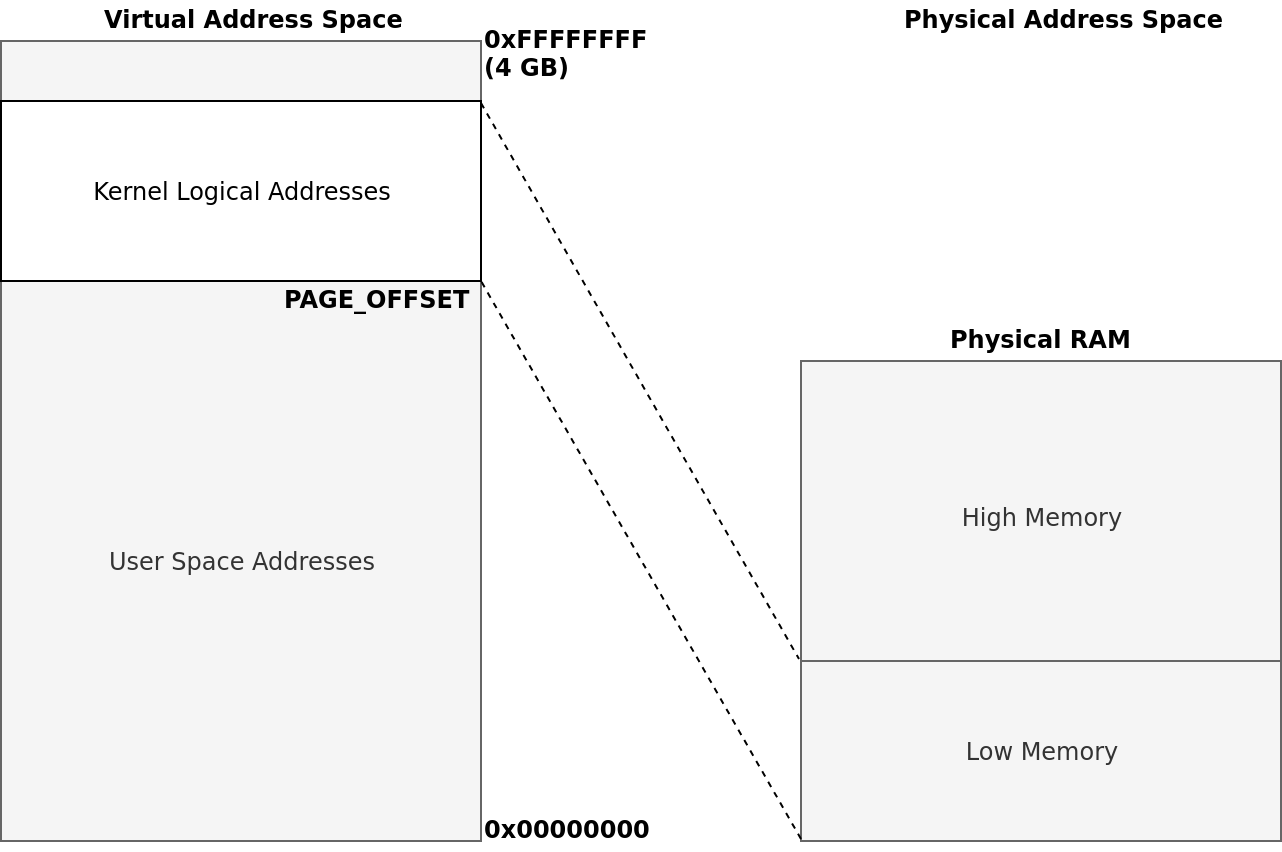
\includegraphics[scale=0.15]{HighLowMem}
	\caption{The relation between virtual and physical memory in 32-bit x86 architectures\cite{lfd430}}\label{pic:high-low-mem}
    %TODO own picture!
\end{figure} \ \\
%
Actually, the division in high and low memory just one from several. 
Linux uses additionally a \textit{zone allocator} memory algorithm to partition its address space more fine granular.
Each zone differs in its usage and comes with own methods to perform basic memory operations like allocate and free memory pages\cite{lfd430}.
On 32-bit x86 architectures, the zones are:
\begin{itemize}
    \item the \textbf{\ac{dma} zone} is located from 0 to 16 MB in both, 32-bit and 64-bit x86 architectures. It must be used for \ac{dma} data transfers on devices with 24-bit addresses.
    \item the \textbf{\ac{dma}32 zone} is also on both variants located from 16 MB up to 4 GB. It must be used for \ac{dma} transfers on devices with 32-bit addresses as suggested by its name.
    \item the \textbf{normal zone} is from 16 MB to 896 MB on 32-bit systems respectively it fills the whole remaining \ac{ram} on 64-bit systems and overlaps with the \ac{dma}32 zone. The normal zone is used for kernel and user data, but kernel addresses in this zone are calculated divergent from user addresses.
    \item the \textbf{high zone} is a 32-bit only facility. It starts from 896 MB and fills the remaining \ac{ram} up to 64 GB. This is also the reason for this special zone: it enables 32-bit x86 systems running on Linux to access more than the usually addressable 4 GB of physical main memory\cite{lfd430}.
\end{itemize}

As suggested, Linux combines its memory management with different types of addresses.
They available types depend on the architecture, too.
This work will focus on 32-bit x86, as usual.
The types are:
\begin{itemize}
    \item \textbf{user virtual addresses} as seen by user space applications. They can be 32 or 64-bit long, even on 32-bit systems and each process has its own virtual address space. As a result, two identical virtual addresses may refer to distinct addresses in the physical memory.
    \item \textbf{physical addresses}, i.e.\ the actual physical memory addresses which are used between the \ac{cpu} and the main memory. Also on this place, the addresses may be 64-bit long, even on a 32-bit system.
    \item \textbf{bus addresses}, which are physical addresses used between the main memory and peripheral buses in x86 architectures. In other architectures or even newer variants, this fact may change.
    \item \textbf{kernel logical addresses}, which are actual physical addresses shifted by an offset. They are always stored in low memory and only used within the Linux kernel itself.
    \item \textbf{kernel virtual addresses}, which are kernel addresses with no need for a direct mapping to physical memory addresses. It is a 32-bit x86 architectural anomaly and not available on 64-bit systems. Kernel virtual addresses which are not logical addresses, too, reside in high memory\cite{lfd430}.
\end{itemize}

\begin{figure} [ht]
	\centering
	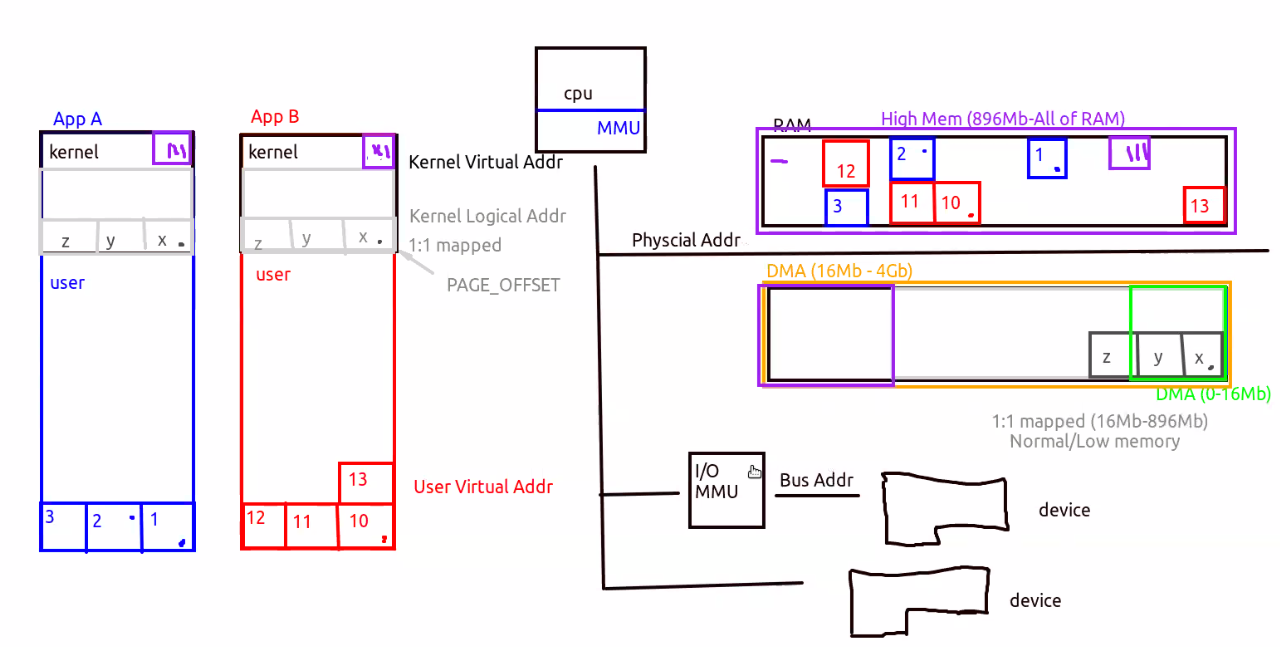
\includegraphics[scale=0.45]{Chapter6-5}
	\caption{Linux memory management overview\cite{lfd430}}\label{pic:linux-mem}
    %TODO own picture!
\end{figure}

As also described in the general section, Linux uses fixed sized pages within memory management.
The actual size of a page depends on the \ac{cpu} architecture.
Pages in x86 are in common 4 KB sized while ARM based architectures may use 4, 16 or 32 KB sized ones. 
Thus, application code should never depend on page sizes.
Linux manages the pages using page tables, too.
For the kernel related pages is the virtual or logical address decoded to the offset and a \textit{virtual \ac{pfn}}.
This \ac{pfn} is stored in the page table together with access control information and a valid flag.
At this point, it becomes apparent that the entire memory handling in Linux and also the protection of memory regions, e.g.\ against writing and/or code execution, is done on page level.
The valid flag indicates if a virtual page is effectively available in main memory. 
If a page is not valid, i.e.\ swapped out to disk or not even yet loaded to the main memory, a \textit{page fault} is raised if the page is requested.
The kernel is invoked to loaded the proper page into main memory using demand paging and the hardware facilities \textit{\ac{mmu}} and \textit{\ac{tlb}}\cite{lfd430}.

Figure~\ref{pic:linux-mem} illustrates the most important terms and concepts of memory management in Linux at a glance.
The graphic is inspired by the one done by \textsc{John Bonesio} during the \textit{Developing Linux Device Drivers} Linux foundation training class.
On the left hand side of the graphic, the view to the (virtual) memory from two distinct applications A and B is pictured.
Both see their own virtual address space using \textit{user virtual addresses}, marked in blue and red.
The view on the kernel's address space is the same for both of them.
On the right hand side, the graphic pictures the connection between \ac{cpu} and \ac{mmu} (including but not pictured the \ac{tlb}),  the physical main memory divided into \textit{low} and \textit{high memory} and the peripherals as well as the address types used in between.
The physical memory is divided into the known memory zones, the \textit{\ac{dma}} zone in green, the \textit{\ac{dma}32 zone} in orange, the \textit{normal zone} or low memory in grey and the \textit{high zone} or high memory in \textit{purple}.
Additionally, the graphic symbolizes how pages in different contexts are mapped into the physical main memory.
Both user processes have numbered pages which can also be found in the right hand side \ac{ram} representation.
Furthermore are some kernel pages marked in grey with the characters \textit{z, y and x} which are 1:1 mapped into the normal memory (kernel logical addresses) and a page in purple (kernel virtual address), mapped into the high memory zone. 

Linux memory management is, as already named, a very complex topic.
This section is only an introduction to the most important terms and concepts.
It is not possible to give a complete and detailed summary on this topic as part of this work.
Thus, a very good and detailed resource to memory management in Linux on different architectures and the effects on kernel programming is the \textit{LFD430 Developing Linux Device Drivers} course script\cite{lfd430} respectively the according Linux foundation training class, which was also used as main source for this section. 
% memory allocation
% in common, a linux (kernel) programmer allocated whole pages of memory
% if less is needed or multiple of the page size does not fit without wasting pages, linux provides the SLAB/SLUB/SLOB allocator scheme
%

\subsection{Memory Management in Zircon} 


\section{I/O}\label{sec:io} 
%TODO review sections, how is it done in Linux/Zircon
\subsection{I/O Hardware}
\subsection{Memory Mapped IO}
\subsection{Direct Memory Access}
\subsection{Interrupts}
\subsection{Power Management}

   
% \section{Security Concepts} %TODO label
% \subsection{Access Control} %Domains, Capabilities
% %DAC, MAC, ..
% \subsection{Security Concepts in Linux}
% \subsection{Security Concepts in Zircon}


%TODO own chapter
\section{Driver Models} %TODO label
